\section{Testing WebRTC}

\thispagestyle{empty}

In this chapter we will study how WebRTC performs in different use cases and topologies previously described in chapter~\ref{sec:topologies}. All tests will be done using a real working environment combining the tools mentioned in chapter~\ref{sec:testingEnv}.

\subsection{Interoperability}

One of the main goals of WebRTC is that it should be interoperable between different browser vendors. In this chapter, we will analyze if it is possible for all browsers to be interoperable.

Actually, three different browsers carry native implementations for WebRTC: Google Chrome, Mozilla Firefox and Opera. Of those, two of them include the {\it GetUserMedia} and {\it PeerConnection} APIs: Mozilla Firefox and Google Chrome, they should be interoperable between them. Google Chrome has included WebRTC {\it PeerConnection} API for long time, but Mozilla Firefox came up with the {\it PeerConnection} API much later~\cite{chromefirefoxinterop}. Making both browsers compatible required work from the vendors, because the SDP messages provided by them are different but rely on the IETF standard. Both engines should be able to understand those signaling messages and respond with the adequate SDP negotiation.

However, there are some differences in the SDP signaling messages, in the Firefox implementation, the implementation provides the STUN/TURN candidates bundled on the message meanwhile the API from Chrome provides the candidates separately by default, at the same time, the signaling messages from Chrome include some extra information about the streams that is not given in the Firefox version~\cite{interopnotes}.

Furthermore, both browsers must implement cross-compatible codecs to send the stream and be able to handle the proper incoming RTP packets. Even though, most compatibility issues are solved, there are still some ongoing problems with the actual JavaScript method calls in both browsers~\cite{interopnotes}.

One of the goals when checking the interoperability of the browsers, is to evaluate the enabled congestion mechanisms already implemented in both APIs. They should be able to manage the different environments in the same way as they rely on top of the same standards. At the time of this document, not all congestion control mechanisms are included in Mozilla Firefox.

For this test we have executed a point-to-point call between a Firefox and Chrome in different machines. We are more interested in seeing the behavior of the call rate and other metrics between the peers than the possible overall averaged result.

\begin{figure}[h]
  \centering
    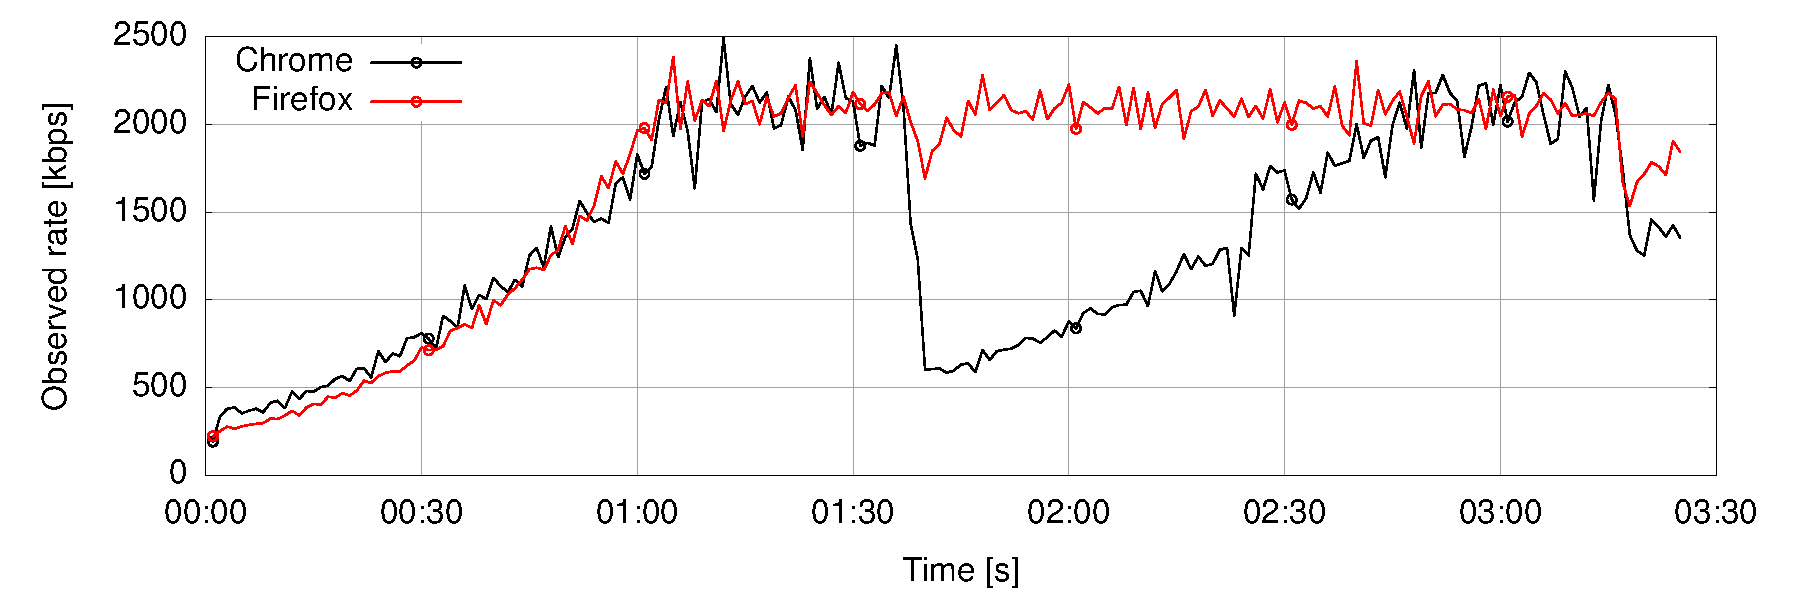
\includegraphics[width=1\textwidth]{./figures/firefoxvschrome1.pdf}
      \caption[Remote stream rate for a point-to-point call between Mozilla Firefox and Google Chrome]{Remote stream rate for a point-to-point call between Mozilla Firefox and Google Chrome.}
	\label{fig:firefoxvschrome1}
\end{figure}

Figure~\ref{fig:firefoxvschrome1} illustrates the rate given by the streams of both vendors captured at each receiver. We can observe that congestion mechanism is not triggered for the Firefox stream when some congestion occur on the path, Chrome applies some rate adaptation meanwhile Firefox maintains the same stream rate over the link.

%Considering that we haven't applied any constraint on the link for this scenario, we could consider this as a misunderstanding between both %transport layers, the delay over the path is barely inexistent and there is no packet loss on the reported metrics.

We should consider that WebRTC should RTCP message with Receiver Estimated Maximum Bitrate (REMB) \nomenclature{REMB}{Receiver Estimated Maximum Bitrate} for rate adaptation~\cite{alvestrandCongestion2012}~\cite{alvestrandCongestionREMB}. This mechanism provides an extra field in the WebRTC RTCP messages with the estimated total available bandwidth for the session. 

%Considering that Firefox has not fully implemented it's congestion mechanism, this mechanism would fail to establish an available rate for both %ends giving this type of unstable output for Chrome which expects this parameter to be available.

%\begin{figure}[h]
%  \centering
%    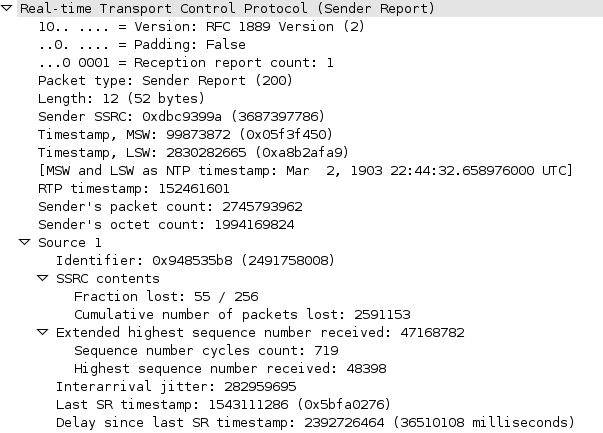
\includegraphics[scale=0.7]{./figures/rtcpchrome.png}
%      \caption[RTCP packet content sent by a Google Chrome WebRTC call]{RTCP packet content sent by a Google Chrome WebRTC call.}
%	\label{fig:rtcpchrometochrome}
%\end{figure}

To check the behavior of the RTCP feedback mechanism in WebRTC, we have captured different samples using a network sniffer. However, it is important to advise that some of the congestion mechanisms are still in ongoing discussion in the working groups and have not reached full consensus.

Firstly, we obtained a capture from a call between two Chrome browsers, after analyzing the data, we can observe that both peers where exchanging {\it Sender Reports} control packets. In WebRTC, the RTT measurement of the RTCP packets is made by using the same RTP media flow timing, this avoids the usage of {\it Receiver Reports} in most point-to-point or single {\it PeerConnection} topologies. WebRTC multiplexes the RTP and RTCP packets in the same port to avoid extra usage of network resources~\cite{rtpusageIETF}.

Those messages carry important data required by the WebRTC internals to build the {\it Stats API}. The following fields (\ref{lst:rtcpchrometochrome}) are extracted from a RTCP packet sent by a Google Chrome browser in our test. We can see that most of the metrics are available in the packet, other required metrics which are not fully standardized as REMB are not able to be decoded by our packet sniffer~\cite{rtpusageIETF}.

\lstset{language=sh}
\begin{lstlisting}[caption={RTCP message exchange between Chrome and Firefox},label={lst:rtcpchrometochrome}]
Real-time Transport Control Protocol (Sender Report)
    10.. .... = Version: RFC 1889 Version (2)
    ..0. .... = Padding: False
    ...0 0001 = Reception report count: 1
    Packet type: Sender Report (200)
    Length: 12 (52 bytes)
    Sender SSRC: 0xdf1a474d (3743041357)
    Timestamp, MSW: 3026830625 (0xb469c521)
    Timestamp, LSW: 653452974 (0x26f2e6ae)
    [MSW and LSW as NTP timestamp: Dec  1, 1995 18:17:05.152143000 UTC]
    RTP timestamp: 973093429
    Sender's packet count: 4236773172
    Sender's octet count: 3803919253
    Source 1
        Identifier: 0x9046a1ac (2420548012)
        SSRC contents
            Fraction lost: 102 / 256
            Cumulative number of packets lost: 4832630
        Extended highest sequence number received: 1896484047
            Sequence number cycles count: 28938
            Highest sequence number received: 3279
        Interarrival jitter: 1420789294
        Last SR timestamp: 2622976836 (0x9c577344)
        Delay since last SR timestamp: 2032955356 (31020436 milliseconds)

Real-time Transport Control Protocol (Receiver Report)
    10.. .... = Version: RFC 1889 Version (2)
    ..0. .... = Padding: False
    ...0 0001 = Reception report count: 1
    Packet type: Receiver Report (201)
    Length: 7 (32 bytes)
    Sender SSRC: 0xf46245fb (4100081147)
    Source 1
        Identifier: 0x7f3343fb (2134066171)
        SSRC contents
            Fraction lost: 217 / 256
            Cumulative number of packets lost: 3472040
        Extended highest sequence number received: 4229724701
            Sequence number cycles count: 64540
            Highest sequence number received: 31261
        Interarrival jitter: 1181356458
        Last SR timestamp: 2930563385 (0xaeacd939)
        Delay since last SR timestamp: 3634988546 (55465523 milliseconds)
\end{lstlisting}

Furthermore, some other features are required to be answered by the WebRTC RTCP engine, but might not be asked by the {\it PeerConnection} if they are not necessary or implemented in one of the peers. This is why features such as REMB may still not provided the RTCP {\it Sender Report}, if this field is not available, the congestion mechanism of Chrome calculates the estimated rate by using the mechanisms provided in the RMCAT Internet-Draft~\cite{alvestrandCongestion2012}, those mechanisms use the information extracted from the RTCP report (\ref{lst:rtcpchrometochrome}). 

During the capture with different vendors we have observed a different behavior in the RTCP mechanisms between Chrome and Firefox. Meanwhile Chrome continuously provide the {\it Sender Report} metrics in the RTP/RTCP channel, Firefox is only reporting {\it Receiver Reports} back to the source, this message exchange procedure is seen in the previous description(\ref{lst:rtcpchrometochrome}). No metrics from the outgoing stream of Firefox are being sent to Chrome, this forces Chrome not to provide any feedback control messages to Firefox that would trigger congestion control mechanisms. This behavior may affect the rate adaptation mechanisms in Firefox which could lead to an output similar to Figure~\ref{fig:firefoxvschrome1}.

We can state that congestion mechanisms on Firefox are still not available and this reject any rate adaptation in Firefox, in conclusion, using Firefox in multiple scenarios would lead to unexpected rate response and poor call quality. Apart from the congestion control mechanisms, Firefox and Chrome APIs are fully interoperable to perform calls even though some features, such as statistics, are still not available. 

\subsection{WiFi scenario}

To check the performance of WebRTC in a wireless scenario we have stablished a simple call between two peers that handle video and audio in an open WiFi network. This network does not carry any UDP packet filter or Firewall, the connection is performed without the need of STUN or TURN, we could easily say it is a straight forward host peer-to-peer connection. The aim of this test is to observe how the captures differ between origin and receiver between {\it StatsAPI} and {\it ConMon}.

 \begin{figure}[h]
  \centering
    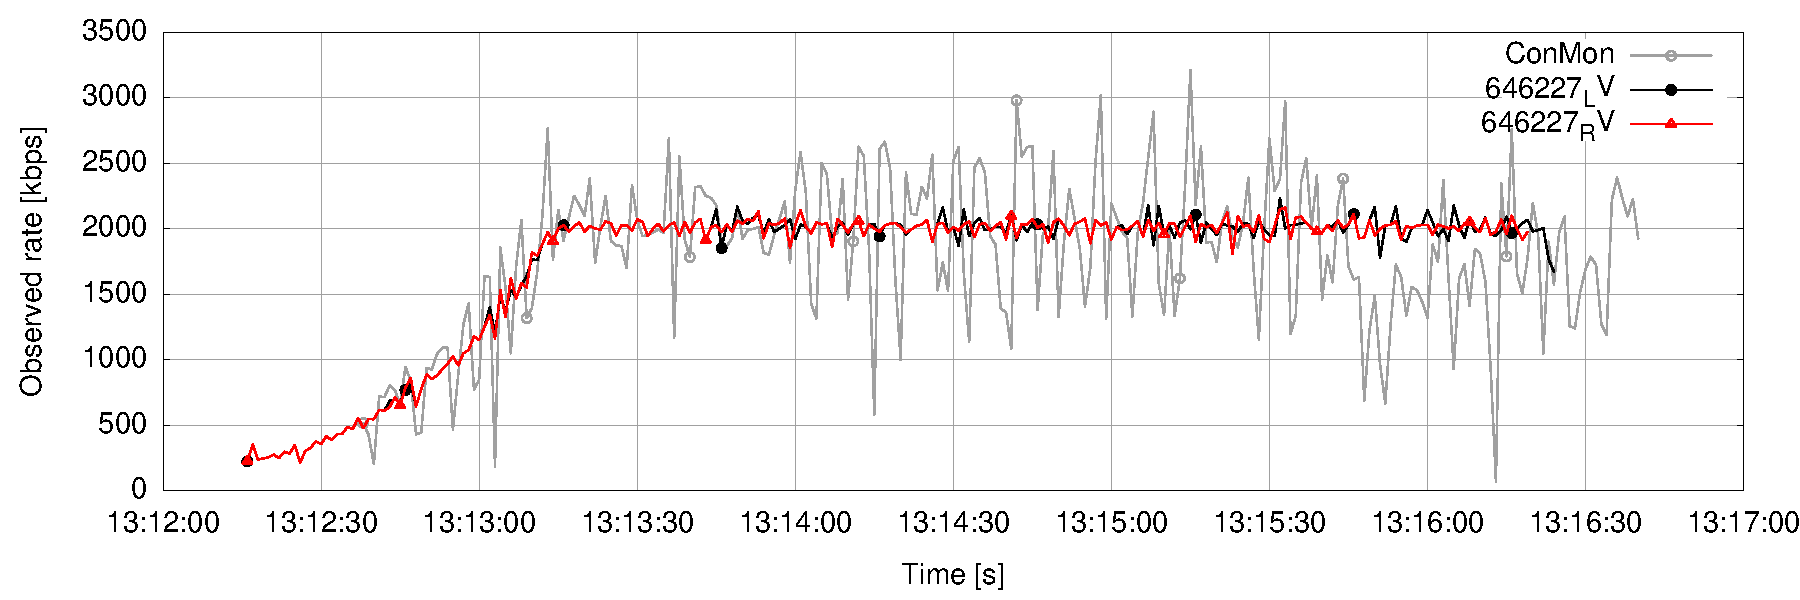
\includegraphics[width=1\textwidth]{./figures/onetoone_wifi_statsconmon.pdf}
      \caption[Point-to-point video stream plot using StatsAPI and ConMon data over WiFi]{Point-to-point video stream plot using StatsAPI and ConMon data over WiFi.}
	\label{fig:onetooneWifistatsconmon}
\end{figure}

Figure~\ref{fig:onetooneWifistatsconmon} represents the throughput rate on the same video stream, the three lines are the comparison between local video stream on the source, remote video stream at the receiver and {\it ConMon} capture of the remote video stream at the receiver. The same stream has been measured from three different perspectives, this will help us to understand the difference of rate that the overhead of the RTP is consuming and the disruption caused by the WiFi network.

Notice that red and black colors represent the Local Video (LV) and Remote Video (RV) from with same SSRC captured using {\it Stats API}, the grey line illustrates the capture performed using {\it ConMon} of the same stream. It is easy to observe that both {\it StatsAPI} captures are similar, some offset is given due to the processing time between the network layer and the browser API that returns all values. Besides this, the capture is smooth and the outgoing and incoming rate of the origin client and input of the receiver are similar. Capture in the network layer using {\it ConMon} is more abrupt as all packets are captured over the WiFi and the period used when plotting affects the moment when value is stored, when having two peaks with opposite they should balance each other, meaning that the transmission in most of the period is stable and the peaks when plotting are a result of post-processing accuracy. Call duration in this test has been around five minutes. Some areas, mostly between 13.15.30 and 13.16.00, show a strange oscillation of the rate that could be produced by the WiFi, this throughput distortion is balanced on the WebRTC layer as the rate delivered to the API does not change.

When we try to measure the quality of the call, one important indicator is the delay of the stream, to calculate the delay we can either use the RTT measured by our {\it Stats API} or the captures performed on the network layer by {\it ConMon}. The {\it ConMon} procedure will give us higher accuracy by subtracting the timestamps from both captures of the same stream in each peer, to obtain a good result in this procedure we might have to reduce the internal clock drift of both peers by using systems such as Network Time Protocol daemon (NTPd) \nomenclature{NTPd}{Network Time Protocol daemon}.

 \begin{figure}[h]
  \centering
    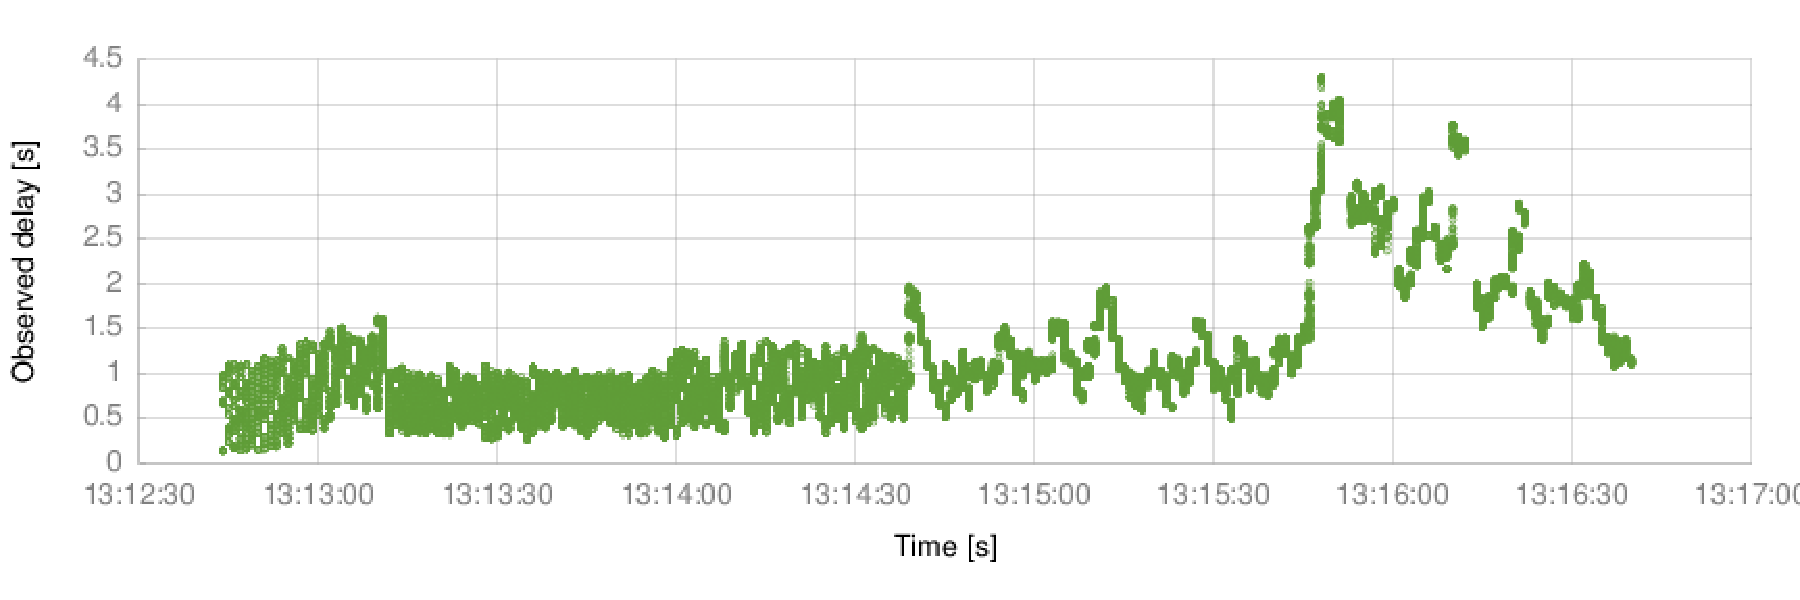
\includegraphics[width=1\textwidth]{./figures/delay_116_646227.pdf}
      \caption[Delay calculated on the same stream captured using ConMon in both ends over WiFi]{Delay calculated on the same stream captured using ConMon in both ends over WiFi.}
	\label{fig:delay_116_646227}
\end{figure}

Figure~\ref{fig:delay_116_646227} represents the delay of the stream plotted in~\ref{fig:onetooneWifistatsconmon}. We can see that the quality of the call is affected by the network distortion at Figure~\ref{fig:onetooneWifistatsconmon}, this variation of the rate delivers a high delay of more than 4 seconds during some periods of the call and an average of approximately 1 second globally, the media received in those periods will not render correctly and the user experience of the call is going to be worst than at the beginning of the call.

WebRTC haven't performed as expected on this scenario providing big delays and low quality media when the status of the link is not optimal.

\subsection{Point-to-point}

In a point-to-point scenario we have performed different tests to calculate how the application performs. 

\subsubsection{Non-constrained link test}

After seeing how WebRTC performs in WiFi  we are going to proceed with all tests in a controlled wired scenario adding different constraints to the link. This tests will be automated running ten iterations every time in order to get as much accurate results as possible.
 
 \begin{figure}[h]
  \centering
    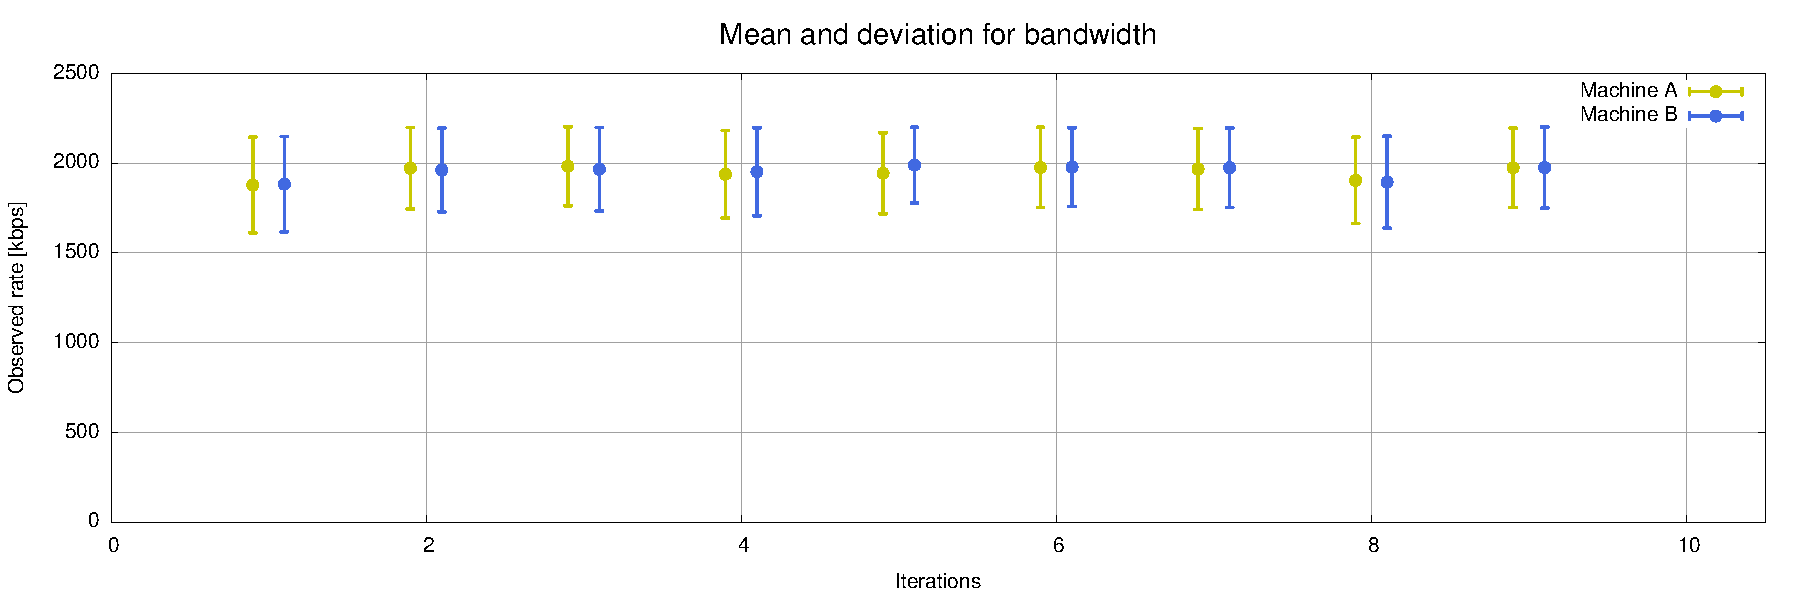
\includegraphics[width=1\textwidth]{./figures/no_ipfw.pdf}
      \caption[Bandwidth results for non-conditioned link]{Bandwidth results for non-conditioned link.}
	\label{fig:no_ipfw}
\end{figure}

Figure~\ref{fig:no_ipfw} plots the average bandwidth of every call in a wired network without any link condition, the average bandwidth obtained in the test is 1949.7 Kbit/s with 233 Kbit/s of deviation which gives the conclusion of having approximately 1 Mbit/s standard bandwidth in a video stream for a non-conditioned link in WebRTC. Delay result in 5.1 ms with 1.5 ms deviation and RTT about 9.5 ms. Those results can be taken as standard for a non-conditioned WebRTC with high bandwidth resources. A summary of results is shown in Table~\ref{fig:p2p_no_ipfw}. Some interesting results to track is the amount of calls failed in every test, considering all those calls go through a TURN server we might be able to approximate the success rate when establishing calls. All results go along with the deviation being this an important factor, in this test without any link conditioner we might have small deviation values such as milliseconds, but when adding conditions to the link those values will grow carrying less accuracy.
Setup time is stablished as the time it take since the start of the PeerConnection object until the media stream from the other peer arrives, this value directly affects the time it takes for a user to be able to start talking, in the optimal environment it takes about 1.5 seconds to start the call. We also had zero packet losses and two calls that failed to succeed using TURN in the standard environment.

\begin{table}[h]
\begin{center}
    \begin{tabular}{c D{,}{\pm}{-1} D{,}{\pm}{-1} D{,}{\pm}{-1} }
   	 \toprule
	\textit{}
	& \multicolumn{1}{c}{\textit{Machine A}}
	& \multicolumn{1}{c}{\textit{Machine B}}
	& \multicolumn{1}{c}{\textit{Overall}}\\
	\midrule
	\textbf{CPU (\%)} & 48.76 ,2.76 & 48.83 ,2.78 & 48.79 ,2.77\\
	\textbf{Memory (\%)} & 35.98 ,0.3 & 36.43 ,0.29 & 36.21 ,0.29\\
	\textbf{Bandwidth (Kbit/s)} & 1947.61 ,232.75 & 1951.76 ,234.5 & 1949.7 ,233.62\\
	\textbf{Setup time (ms)} & 1436.33 ,25 & 1447.44 ,22.71 & 1441.88 ,24.04\\
	\textbf{RTT (ms)} & 9.49 ,2.11 & 9.64 ,2.71 & 9.57 ,2.41\\
	\textbf{Delay (ms)} & 4.84 ,1.5 & 5.4 ,1.53 & 5.12 ,1.52\\
	\bottomrule
    \end{tabular}
    \caption[P2P test with no link conditions]{P2P test with no link conditions.}
    \label{fig:p2p_no_ipfw}
\end{center}
\end{table}

Delay values in Table~\ref{fig:p2p_no_ipfw} are represented as a mean calculation of all the delay obtained in the link, thus this value is not representative of what happened in the call. Considering the example in Figure~\ref{fig:delay_116_646227} we can see that the delay can variate during the call being the mean not appropriate to measure the response against the conditions of the link. In order to observe the behavior of WebRTC in delay we have two different approaches, the mean delay with deviation and delay distribution of all calls. 

 \begin{figure}[h]
  \centering
    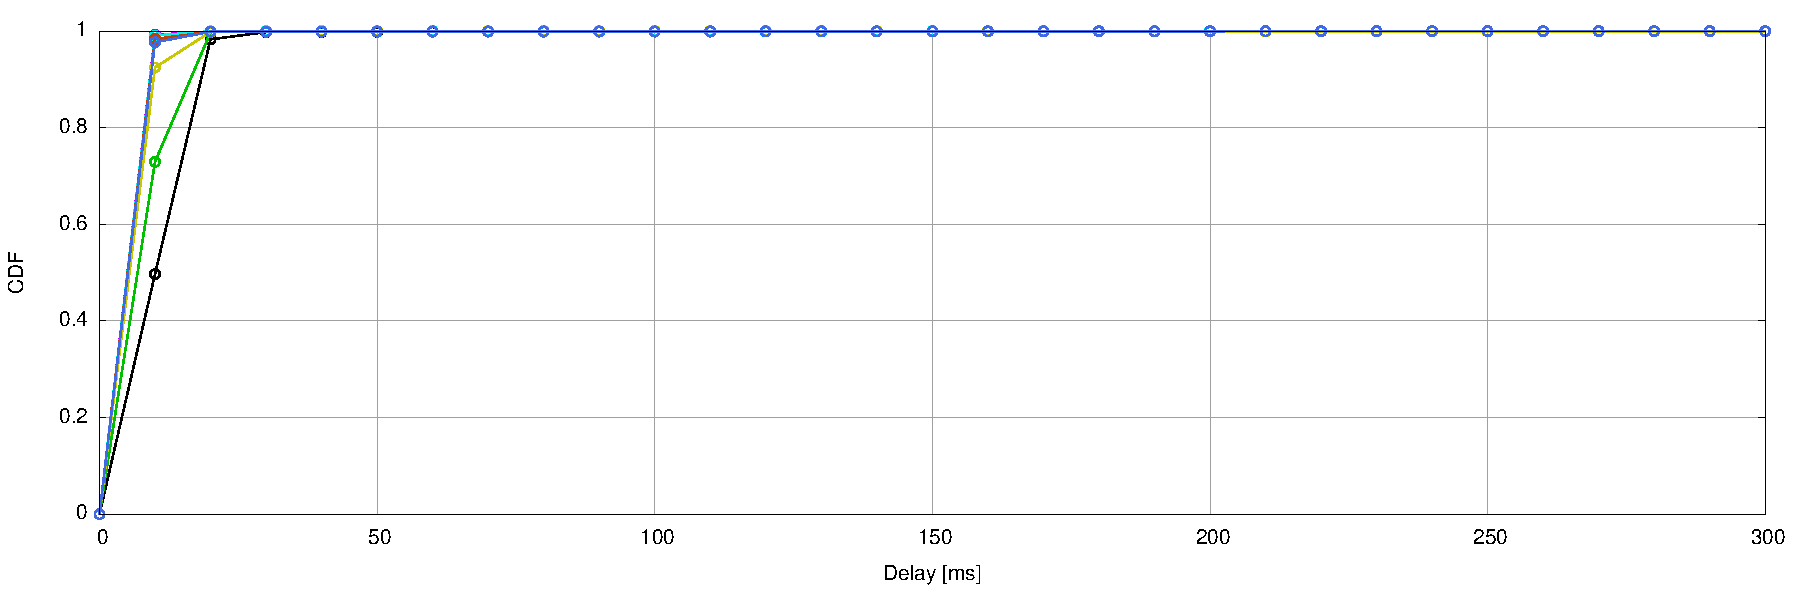
\includegraphics[width=1\textwidth]{./figures/total_delay_distribution_no_ipfw.pdf}
      \caption[Delay distribution in each P2P iterations with no link constraints]{Delay distribution in each P2P iterations with no link constraints.}
	\label{fig:total_delay_distribution_no_ipfw}
\end{figure}

 \begin{figure}[h]
  \centering
    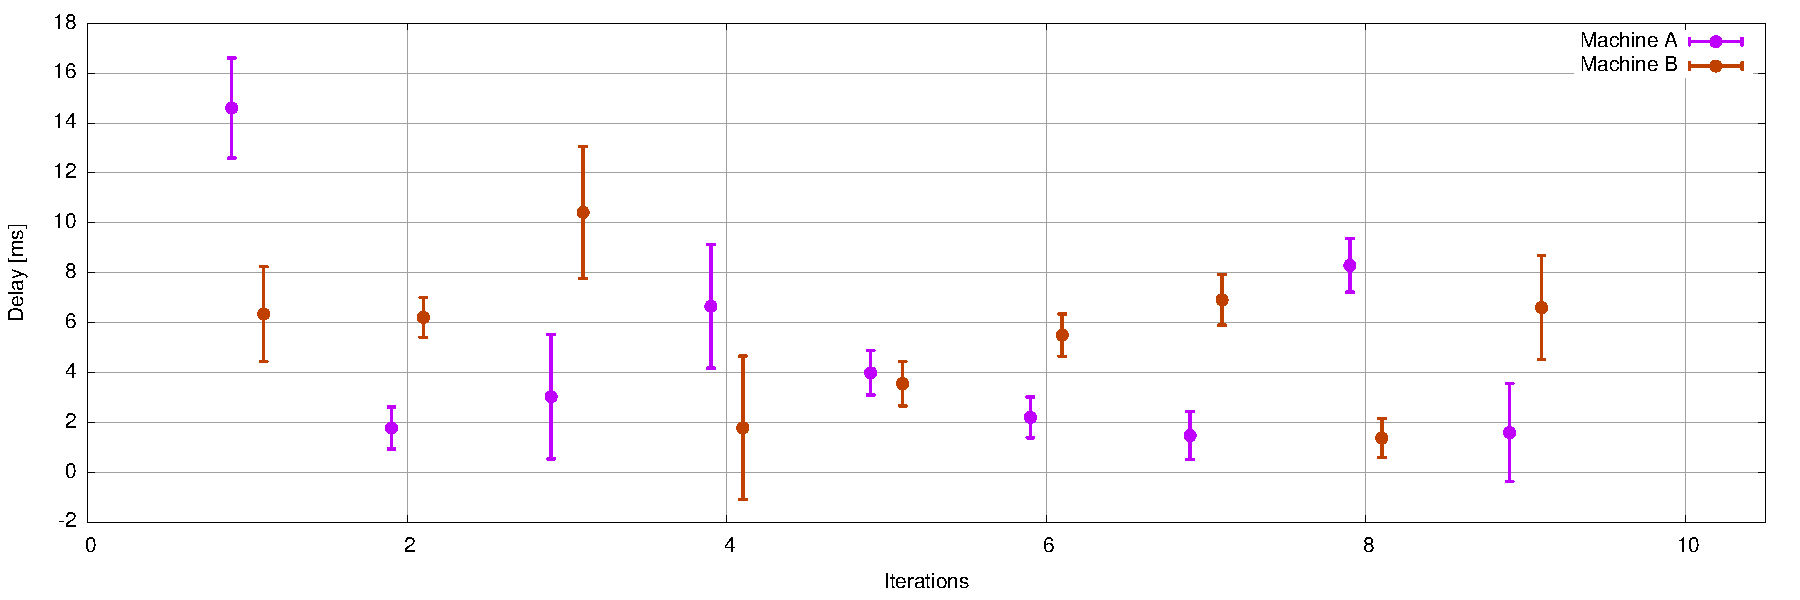
\includegraphics[width=1\textwidth]{./figures/mean_deviation_delay_no_ipfw.pdf}
      \caption[Bandwidth mean and deviation for delay in each P2P iterations with no link constraints]{Mean and deviation for delay in each P2P iterations with no link constraints.}
	\label{fig:mean_deviation_delay_no_ipfw}
\end{figure}

Figure~\ref{fig:mean_deviation_delay_no_ipfw} represents the mean and deviation of delay calculated for all iterations, this delay is calculated on basis with the arrival timestamp for each packet with the captures performed in both sides by {\it ConMon}. We run an NTPD daemon to calculate the drift on the time and sync both machines.  There is small amount of drift of maximum 3ms in the worst case and as small as 1ms in the best one. In Figure~\ref{fig:total_delay_distribution_no_ipfw}, the distribution is given by the amount of packets that have some specific amount of delay, they are counted by batches of 10ms with a maximum range of 300ms. Most of the packets run with less than 25ms delay in all the iterations. The user experience with this small amount of delay with no aggressive steps in the plot will be barely negligible. Figures~\ref{fig:mean_deviation_delay_no_ipfw} and~\ref{fig:total_delay_distribution_no_ipfw} differentiate from Figure~\ref{fig:delay_116_646227} in the measurement of a global delay for an specific constraint scenario instead of just plotting a single call case, many aspects may affect the delay and the an optimal way to observe it is to plot the distribution and deviation of each iteration and try to guess a patron that repeats, Figure~\ref{fig:delay_116_646227} is good to observe just one call if we add some conditions to the link meanwhile the call is going on.

\subsubsection{Behavior in lossy environments}

We have performed some tests regarding lossy environments to see how WebRTC behaves in those, lossy situations can be given with some mobile environments with low coverage or just by having a busy link with no resources available.

We have tested the topology with 1, 5, 10 and 20\% of packet loss, according to the results in Table~\ref{fig:p2p_packet_bw} we are seeing a pretty good response from the internal algorithm up to 5\% with small effect to the bandwidth and delay. When running with 10\% loss the bandwidth drops to an average of 1140.8 Kbit/s and 162 Kbit/s deviation which is half of the corresponding amount for an standard call, this affects the quality of the link and video, 20\% loss will affect to the performance dropping the bandwidth to an average of 314.4 Kbit/s with 62 Kbit/s deviation. We can say that the video quality will be worst with lossy networks but the delay is not affected, having a delay distribution response that matches the standard case without affecting the way users will talk, quality will be worst but the call will be correct in terms of usage. All metrics are in the normal range except bandwidth.

The algorithm used in WebRTC regarding to packet loss is proven to work fine in lossy environments with the results obtained, but there is a big gap of performance in the 10\% loss network compared to the results with 20\%, it is obviously a big amount of packets but the response with 20\% is significantly better than the one with 10\%.

\begin{table}[h]
\begin{center}
    \begin{tabular}{c D{,}{\pm}{-1} D{,}{\pm}{-1} D{,}{\pm}{-1} }
   	 \toprule
	\textit{}
	& \multicolumn{1}{c}{\textit{Machine A}}
	& \multicolumn{1}{c}{\textit{Machine B}}
	& \multicolumn{1}{c}{\textit{Overall}}\\
	\midrule
	\textbf{1\% (Kbit/s)} & 1913.59 ,252.11 & 1880.24 ,261.46 & 1896.91 ,256.78\\
	\textbf{5\% (Kbit/s)} & 1609.65 ,158.46 & 1527.84 ,198.59 & 1568.74  ,178.52\\
	\textbf{10\% (Kbit/s)} & 1166.70 ,145.96 & 1114.94 ,177.88 & 1140.82 ,161.92\\
	\textbf{20\% (Kbit/s)} & 333.34 ,65.99 & 295.46 ,57.98 & 314.4 ,61.98\\
	\bottomrule
    \end{tabular}
    \caption[Averaged bandwidth with different packet loss conditions]{Averaged bandwidth with different packet loss conditions.}
    \label{fig:p2p_packet_bw}
\end{center}
\end{table}

The amount of packets lost in every test is slightly lower than the exact percentage of loss because the use of Forward Error Correction in WebRTC in Chrome, this mechanism is used to control errors in data connection with noisy channels that led to packet losses. FEC is not a must feature to implement in WebRTC but Chrome carries it as default.

When using FEC the sender encodes the message in a redundant way, by having this redundancy the receiver is able to detect a limited number of errors and autocorrect those errors without requiring retransmission.

On the other side, the sender calculates its rate based on the receive report that arrives from the receiver, if this report is not received within two times the maximum interval WebRTC congestion mechanism will consider that all packets during that period have been lost halving the rate in the sender. In order to improve response in lossy environments we could consider calculating the optimal value for this interval considering all the possible situations. Considering the congestion algorithm in WebRTC~\cite{alvestrandCongestion2012}, the rate should not vary when having between 2-10\% of packet losses. Table~\ref{fig:p2p_packet_bw} proves that this mechanism is not working properly as we are noticing reduction of rate with 5\% of packet losses, the mechanism should start modifying the rate above 10\% of packet lost calculating a new sender available bandwidth (A$_{\textrm{s}}$) using Equation~\ref{eq:RateCalc} being {\it p} the packet loss ratio.

\begin{equation}
	A_s ( i ) = A_s ( i - 1 ) \times (1 - \frac{p}{2}) 
	\label{eq:RateCalc}
\end{equation}

If the packet loss is less than 2\% the increase of bandwidth will be given by Equation~\ref{eq:RateCalc2}.

\begin{equation}
	A_s ( i ) = 1.05 \times (A_s ( i - 1 ) + 1000) 
	\label{eq:RateCalc2}
\end{equation}

\subsubsection{Delayed networks}

Another interesting situation that are given in mobile environments and queued networks is delay, we have also tested the performance of WebRTC in those conditions. We have benchmarked tests in different one-way delays, 50, 100, 200 and 500ms. In our case, the RTT results should be multiplied by two.

Delay modeling for real time applications is difficult and can be done using the timestamp of the incoming packets, the incoming frame will be delayed if the arrival time difference is larger than the timestamp difference compared to its predecessor frame.

We have noticed that the system performs badly when having even small delays up to 100ms. The response of WebRTC is to reduce the bandwidth by discarding packets, this means that the congestion control systems that act in those environments are not working correctly. On the other hand, delay output does behave correctly having a continuous delay of the according time configured in the constraints, there are no sudden increases of delay and the deviation in delay fits in the standard limits.

Table~\ref{fig:p2p_delay_bw} represents the bandwidth response to the delay conditions, it is interesting to see that the deviation with the biggest delay is smaller than expected. Only with 50ms the system will output a good quality call, when increasing delay the performance of the video will decrease. WebRTC uses VP8 codec which degrades gracefully the quality in packet loss and delay conditions but the response in this case should be better if the congestion mechanisms worked properly.

\begin{table}[h]
\begin{center}
    \begin{tabular}{c D{,}{\pm}{-1} D{,}{\pm}{-1} D{,}{\pm}{-1} }
   	 \toprule
	\textit{}
	& \multicolumn{1}{c}{\textit{Machine A}}
	& \multicolumn{1}{c}{\textit{Machine B}}
	& \multicolumn{1}{c}{\textit{Overall}}\\
	\midrule
	\textbf{50ms (Kbit/s)} & 1909.31 ,258.09 & 1917.81 ,251.62 & 1913.56 ,254.86\\
	\textbf{100ms (Kbit/s)} & 1516.07 ,263.43 & 1453.94 ,272.79 & 1485 ,268.11\\
	\textbf{200ms (Kbit/s)} & 503.71 ,116.45 & 617.92 ,142.69 & 560.82 ,129.57\\
	\textbf{500ms (Kbit/s)} & 303.58 ,59.22 & 207.77 ,32.48 & 255.67 ,45.85\\
	\bottomrule
    \end{tabular}
    \caption[Summary of averaged bandwidth with different delay conditions]{Summary of averaged bandwidth with different delay conditions.}
    \label{fig:p2p_delay_bw}
\end{center}
\end{table}

We can also observe that every iteration follows a different pattern even having an averaged result, Figure~\ref{fig:mean_deviation_bw_delay200} show the test performed at 200ms and the iterations that fail to keep a constant rate making the amount of artifacts in the video affect the quality of the call. We can certainly confirm that the methods that WebRTC should use to control the congestion in the call are not working as they should.

 \begin{figure}[h]
  \centering
    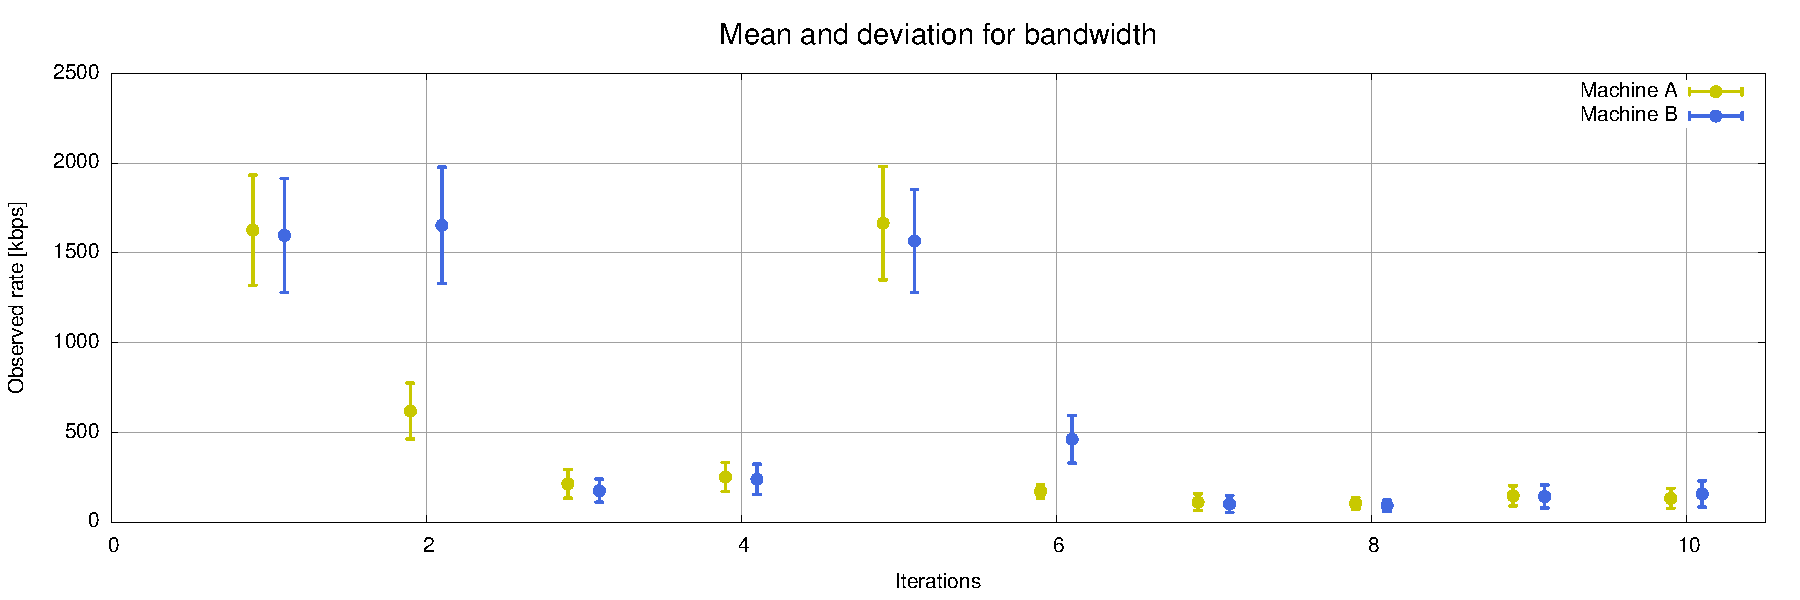
\includegraphics[width=1\textwidth]{./figures/mean_deviation_bw_delay200.pdf}
      \caption[Bandwidth mean and deviation for P2P 200 ms delay test]{Mean and deviation for P2P 200 ms delay test.}
	\label{fig:mean_deviation_bw_delay200}
\end{figure}

The problem with WebRTC relies in the usage of RTP over UDP for packet transport as UDP does not carry congestion control mechanisms that TCP does, when having real time media adapting the encoding to accommodate the varying bandwidth is difficult and cannot be done rapidly.

Low latency networks will play a big role when WebRTC extends to mobile devices and the ability to react properly to delays and packet losses will be crucial for the success of WebRTC in those environments against its competitors.

\subsubsection{Loss and delay}

Regarding P2P scenario we also tested the possibility of having a combined lossy network with delay added to it, this kind of environment could be easily found in mobile applications in low coverage areas. We have set 10\% packet loss with different delays such as 25ms, 50ms, 100ms and 200ms. In Table~\ref{fig:p2p_packet_bw} we saw an average of over 1 Mbit/s of bandwidth usage in 10\% loss environments, the result when adding delay to the constraint is  an average of barely 60 Kbit/s. Those results differ due to the difficulty of WebRTC to handle congestion in those environments. 

\begin{table}[h]
\begin{center}
    \begin{tabular}{c D{,}{\pm}{-1} D{,}{\pm}{-1} D{,}{\pm}{-1} }
   	 \toprule
	\textit{}
	& \multicolumn{1}{c}{\textit{Machine A}}
	& \multicolumn{1}{c}{\textit{Machine B}}
	& \multicolumn{1}{c}{\textit{Overall}}\\
	\midrule
	\textbf{25ms (Kbit/s)} & 72.59 ,18.54 & 70.69 ,18.09 & 71.78 ,18.32\\
	\textbf{50ms (Kbit/s)} & 59.7 ,16.84 & 60.36 ,18 & 60.03 ,17.42\\
	\textbf{100ms (Kbit/s)} & 63.3 ,19.29 & 64.82 ,20.95 & 64.06 ,20.12\\
	\textbf{200ms (Kbit/s)} & 66.89 ,20.12 & 65.66 ,19.63 & 66.27 ,19.87\\
	\bottomrule
    \end{tabular}
    \caption[Averaged bandwidth with different delay conditions with 10\% packet loss]{Averaged bandwidth with different delay conditions with 10\% packet loss.}
    \label{fig:p2p_delay_loss_bw}
\end{center}
\end{table}

Table~\ref{fig:p2p_delay_loss_bw} describes the averaged bandwidth result with not much difference in each situation.If we study the way WebRTC calculates the rate in difficult situations we can see that the sender will establish its decision on the RTT, packet loss and available bandwidth that is estimated from the receiving side using Equation~\ref{eq:RateCalc}~\cite{alvestrandCongestion2012}. Obviously the real output differs form the expected by using the formula, the reason is that even the congestion mechanism on WebRTC calculates the rate using Equation~\ref{eq:RateCalc}, the sender rate is always limited by the TCP Friendly Rate Control (TFRC) formula that is calculated using delay an packet loss ratio together~\cite{tfrc}.

 \begin{figure}[h]
  \centering
    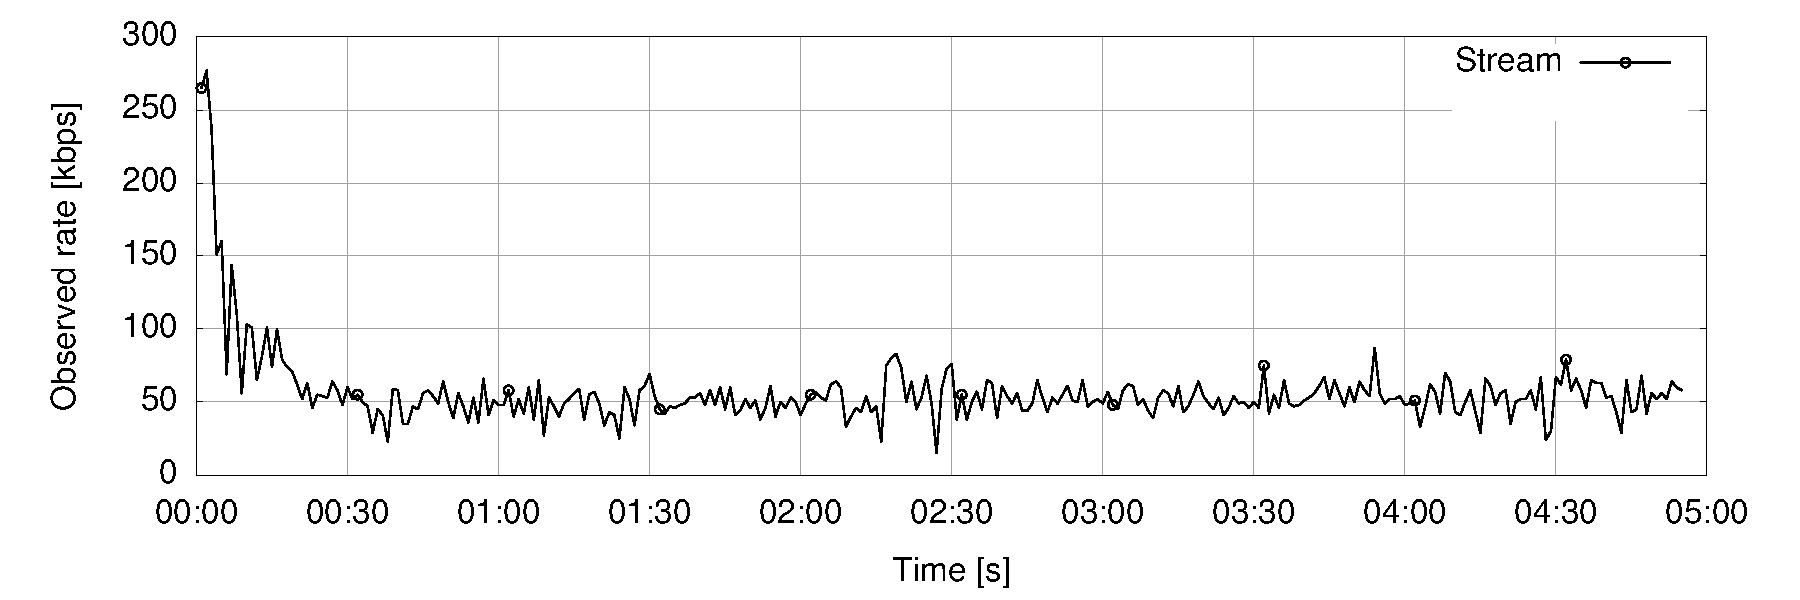
\includegraphics[width=1\textwidth]{./figures/plr10_rtt50ms_RV.pdf}
      \caption[Remote stream bandwidth for 10\% packet loss rate and 50ms delay]{Remote stream bandwidth for 10\% packet loss rate and 50ms delay.}
	\label{fig:bw_plr10_rtt50ms}
\end{figure}

Figure~\ref{fig:bw_plr10_rtt50ms} is an example that illustrates how the rate is lowered after the beginning of the call even the bandwidth is available. This is due to the formulas and mechanisms previously described.

Carrying delay and losses in the same path will not be handled by the congestion mechanisms in WebRTC giving a low rate output for the stream.

Another interesting factor around this test is the setup time that increases to up 4.6 seconds with 200ms delay and 3 seconds with 50ms, obviously this increase will also affect mobile developers when establishing calls in delayed environments.

\subsubsection{Bandwidth and queue variations}

We have also performed a different set of tests modifying the bandwidth and queue length. For this part of the test we have chosen to run 500 Kbit/s, 1, 5 and 10 Mbit/s with different queue sizes ranging from 100 ms, 500 ms, 1s and 10 s. In total we have run 12 different tests with ten iterations each.

The queue size is set in slots to {\it Dummynet} considering each slot as standard ethernet packet of 1500 Bytes, to calculate this number we use Equation~\ref{eq:QueueSize}.

\begin{equation}
	\frac{Bandwidth (Bits)}{8 \times 1500} \times Queue (seconds)
	\label{eq:QueueSize}
\end{equation}

We have seen a good response when having big queue sizes but larger deviation in bandwidth when reducing this queue size to 100 ms or 500 ms, this produced high delays over 20 ms for every call with different distribution curves. The delay that is given to the duration of the call is not stable and will affect the media flow, this increasing curve of delay distribution is given by the small queue size which produces bursty packets to arrive to the peer having different delay conditions.

When we tested the 5 Mbit/s case we got a high delay output even the bandwidth response adapted to the constraints, delay deviation is also high and will affect the time the packets arrive with large jittering.

We will study the result of the test performed at 1 Mbit/s limitation as the maximum standard bandwidth for WebRTC is approximately 2 Mbit/s, when having 1 Mbit/s limitation WebRTC will need to adapt the actual encoding rate and bandwidth control to that amount.

Figure~\ref{fig:1mb_mean_deviation_bw} represents the bandwidth and mean plotted for all the different tests performed in the 1 Mbit/s case. We can see that the response varies in small amount of bandwidth but with large deviation, when having 500ms and 1s queue size (\ref{fig:1mb_500ms_mean_deviation_bw}) we have much more deviation in means of packets being buffered in the relay. Otherwise, when the queue size reduces to 100ms (\ref{fig:1mb_01s_mean_deviation_bw}) the deviation gets smaller but delay response is worst.

We can compare Figure~\ref{fig:1mb_total_delay_distribution} delay distribution results for the best case (\ref{fig:1mb_10s_total_delay_distribution}) and worst case (\ref{fig:1mb_01s_total_delay_distribution}). The delay response with large queue is better due to the rapid increase of packets that carry small delay, for the 100ms queue the curve is smoother having packets ranging in all values of delay between 0 and 130ms.

Delay experience with small queue sizes will be worst in the sense of the call flow, we might experience sudden delay situations that WebRTC won't be able to handle, when having larger queue sizes we son't notice the delay variations as much as with the previous example. Having a curvy increase in delay distribution figure will result in sudden delay variations in the call. The conclusion is that WebRTC is able to adapt to low capacity networks using its codec mechanism at the same time as it should improve the congestion control systems to adapt to different buffer sizes and queuing conditions. 

The congestion mechanisms in WebRTC will stabilize the rate until the amount of delay triggers the rate change to fit the new queue state requirements. Figure~\ref{fig:1cd81aa8-bw} and~\ref{fig:1cd81aa8-delay} show the bandwidth and delay for the same stream and how the rate adapts once the queues are full increasing the delay on the packets, rate is lowered and queues get empty giving producing low delay.

 \begin{figure}[h]
  \centering
    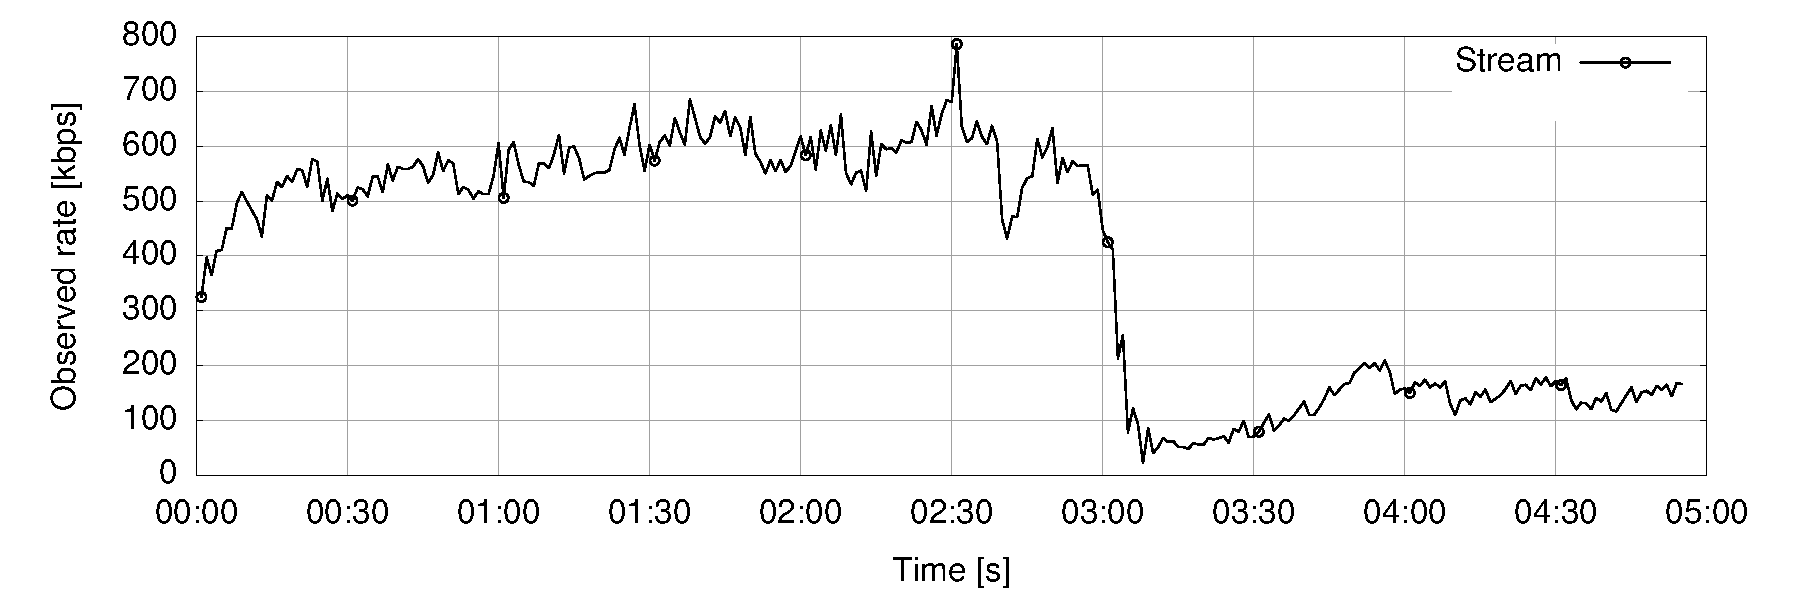
\includegraphics[width=1\textwidth]{./figures/1cd81aa8-bw.pdf}
      \caption[Remote stream bandwidth for 1 Mbit/s and 500ms queue size]{Remote stream bandwidth for 1 Mbit/s and 500ms queue size.}
	\label{fig:1cd81aa8-bw}
\end{figure}

 \begin{figure}[h]
  \centering
    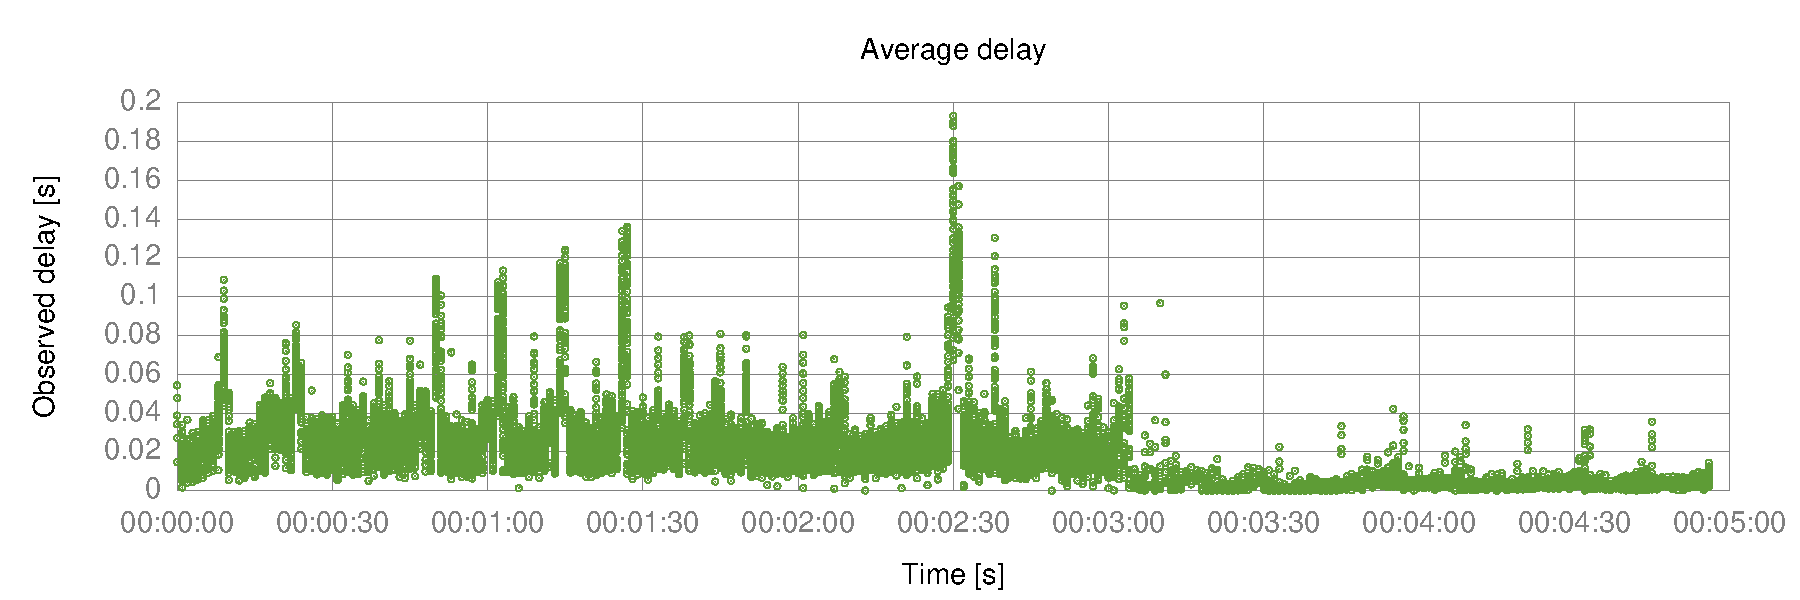
\includegraphics[width=1\textwidth]{./figures/1cd81aa8-delay.pdf}
      \caption[Stream delay for 1 Mbit/s and 500ms queue size]{Stream delay for 1 Mbit/s and 500ms queue size.}
	\label{fig:1cd81aa8-delay}
\end{figure}

Studying the way the sender takes decisions about rate constraints we can observe that the available bandwidth estimates calculated by the receiving side are only reliable when the size of the queues along the channel are large enough~\cite{alvestrandCongestion2012} . When having short queues along the path the maximum usage of the bandwidth cannot be estimated if there is no packet loss in the link, as in this case the packet loss is negligible, the connection is not able to use the maximum amount of bandwidth available in the link.


%Table for all tests
\begin{tabular}{ |c|c|c|c|c| }
\hline
Throughput & Queue & Bandwidht (Kbit/s) & Delay (ms) & Packet Loss (\%)\\ \hline
\multirow{4}{*}{500 Kbit/s} & 100ms & Lucus Radebe & blah & blah\\ \cline{2-5}
 & 500ms & Michael Duberry & blah & blah \\ \cline{2-5}
 & 1s & Dominic Matteo & blah & blah \\ \cline{2-5}
 & 10s & Didier Domi & blah & blah \\ \hline
\multirow{4}{*}{1 Mbit/s} & 100ms & Lucus Radebe & blah & blah\\ \cline{2-5}
 & 500ms & Michael Duberry & blah & blah \\ \cline{2-5}
 & 1s & Dominic Matteo & blah & blah \\ \cline{2-5}
 & 10s & Didier Domi & blah & blah \\ \hline
\multirow{4}{*}{5 Mbit/s} & 100ms & Lucus Radebe & blah & blah\\ \cline{2-5}
 & 500ms & Michael Duberry & blah & blah \\ \cline{2-5}
 & 1s & Dominic Matteo & blah & blah \\ \cline{2-5}
 & 10s & Didier Domi & blah & blah \\ \hline
\end{tabular}

\begin{figure}[htp]
        \centering
        \begin{subfigure}[b]{1\textwidth}
                \centering
                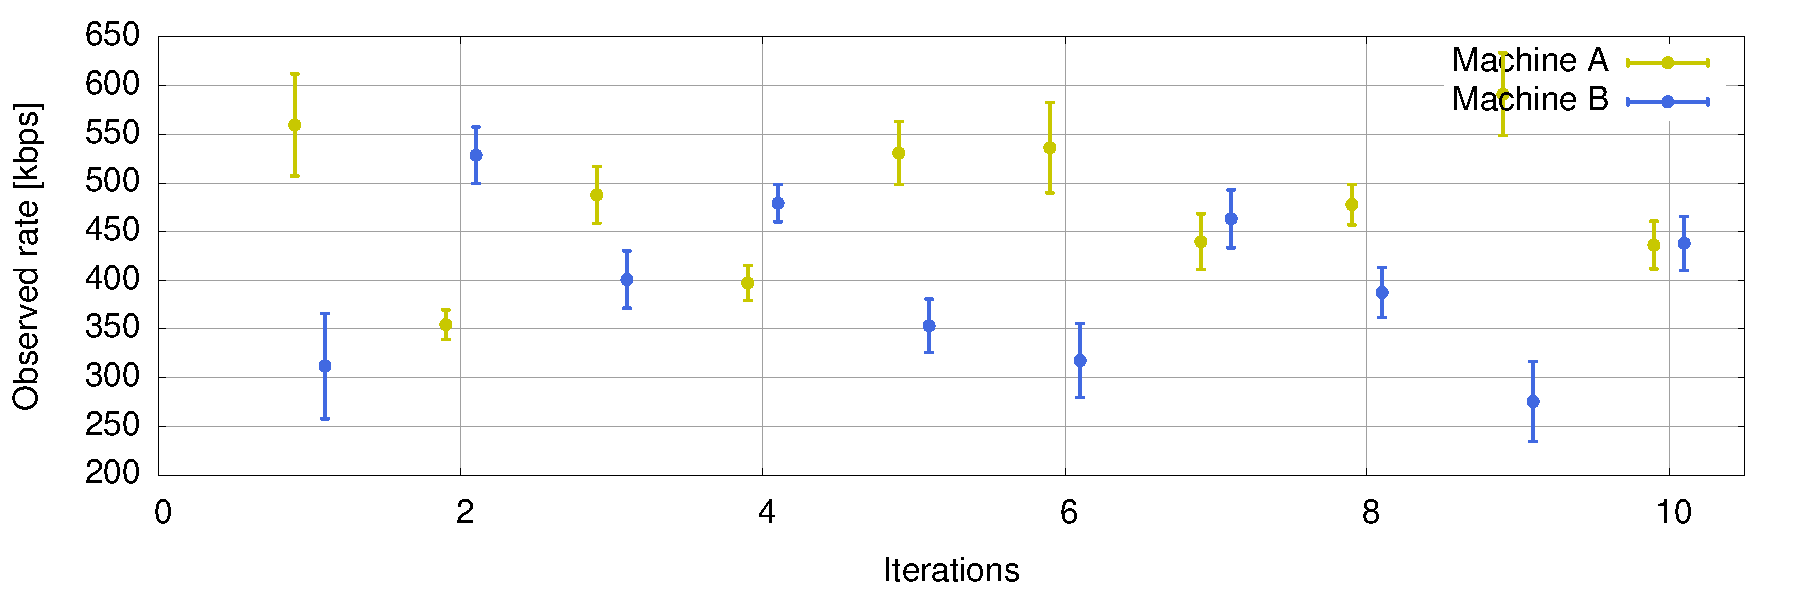
\includegraphics[width=\textwidth]{./figures/1mb_10s_mean_deviation_bw.pdf}
      \caption[1 Mbit/s and 10s queue size]{1 Mbit/s and 10s queue size.}
	\label{fig:1mb_10s_mean_deviation_bw}
        \end{subfigure}
        \qquad

        \begin{subfigure}[b]{1\textwidth}
                \centering
                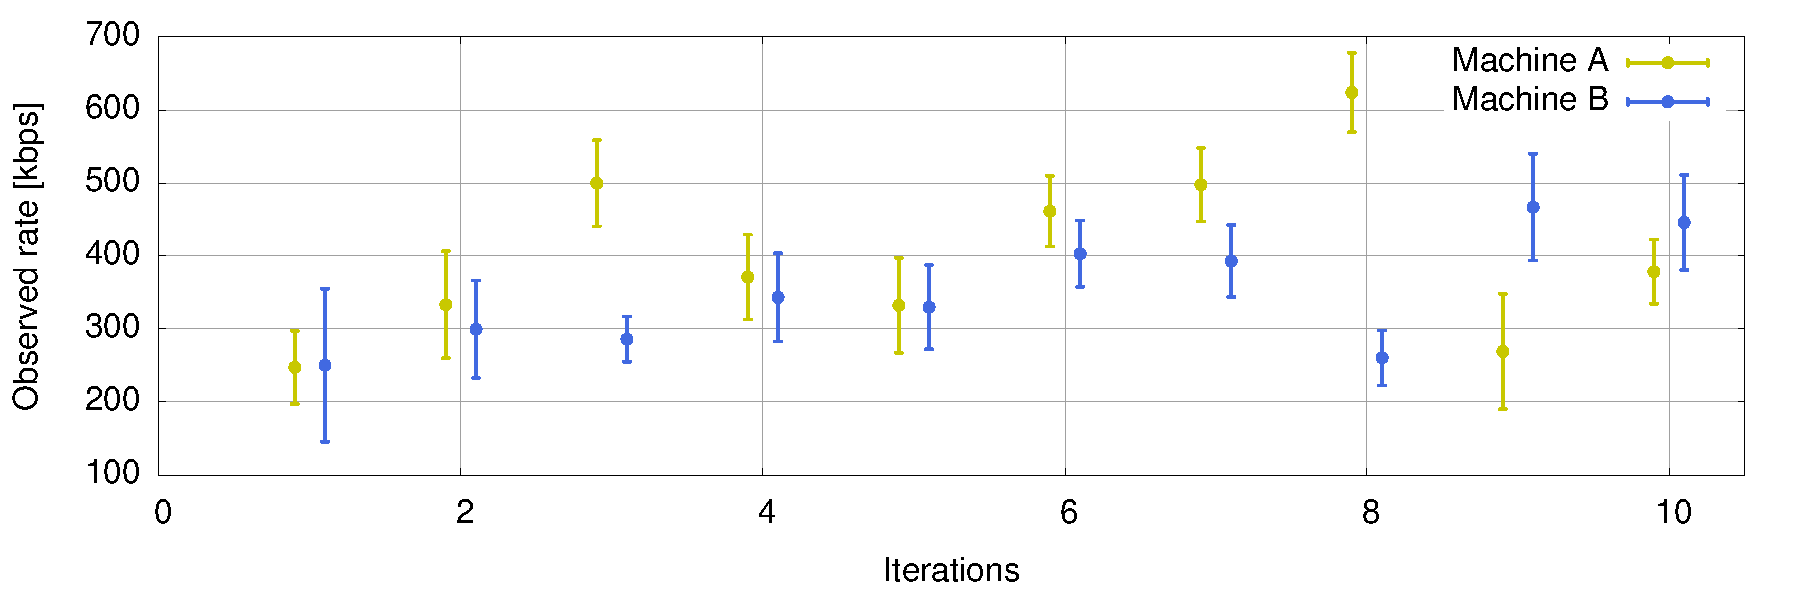
\includegraphics[width=\textwidth]{./figures/1mb_1s_mean_deviation_bw.pdf}
      \caption[1 Mbit/s and 1s queue size]{1 Mbit/s and 1s queue size.}
	\label{fig:1mb_1s_mean_deviation_bw}
        \end{subfigure}
        
        \begin{subfigure}[b]{1\textwidth}
                \centering
                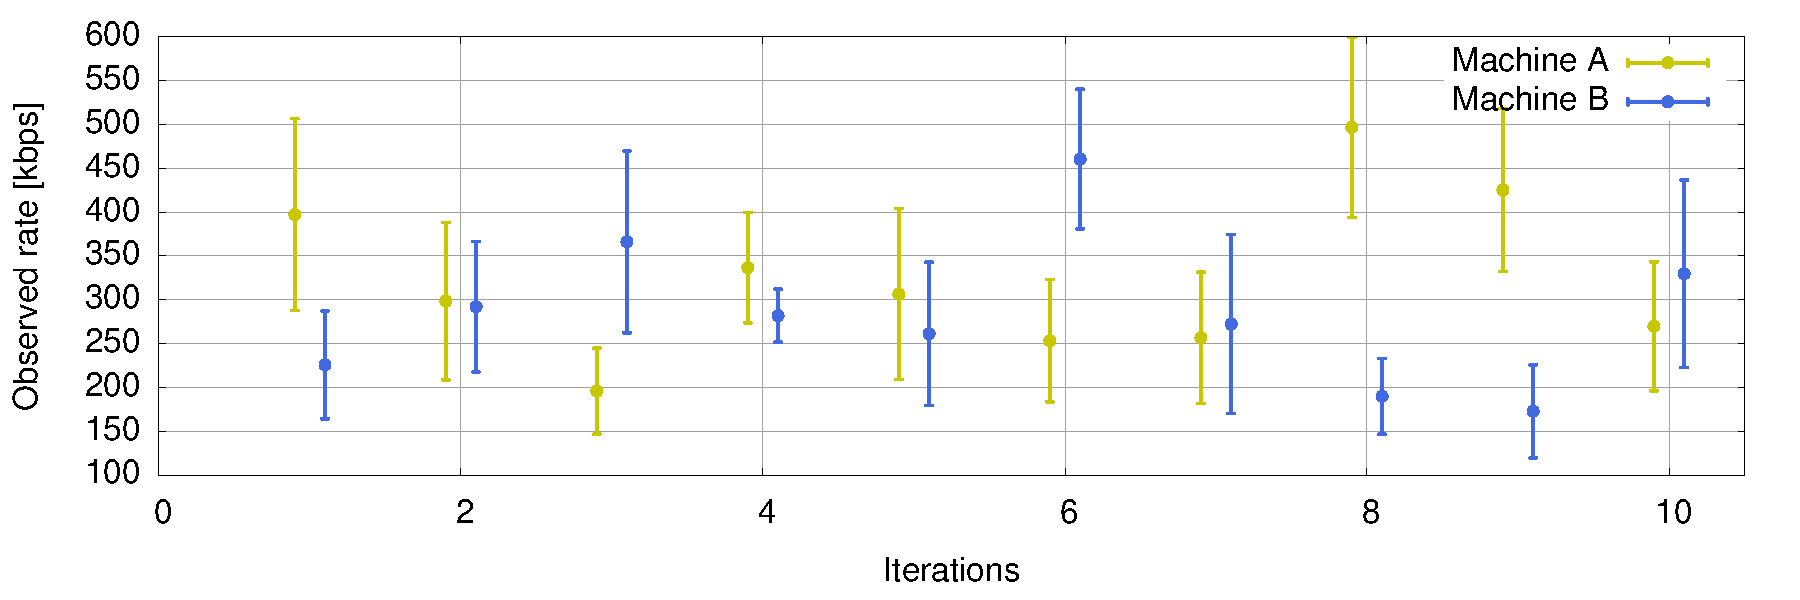
\includegraphics[width=\textwidth]{./figures/1mb_05s_mean_deviation_bw.pdf}
      \caption[1 Mbit/s and 500ms queue size]{1 Mbit/s and 500ms queue size.}
	\label{fig:1mb_500ms_mean_deviation_bw}
        \end{subfigure}
        \qquad

        \begin{subfigure}[b]{1\textwidth}
                \centering
                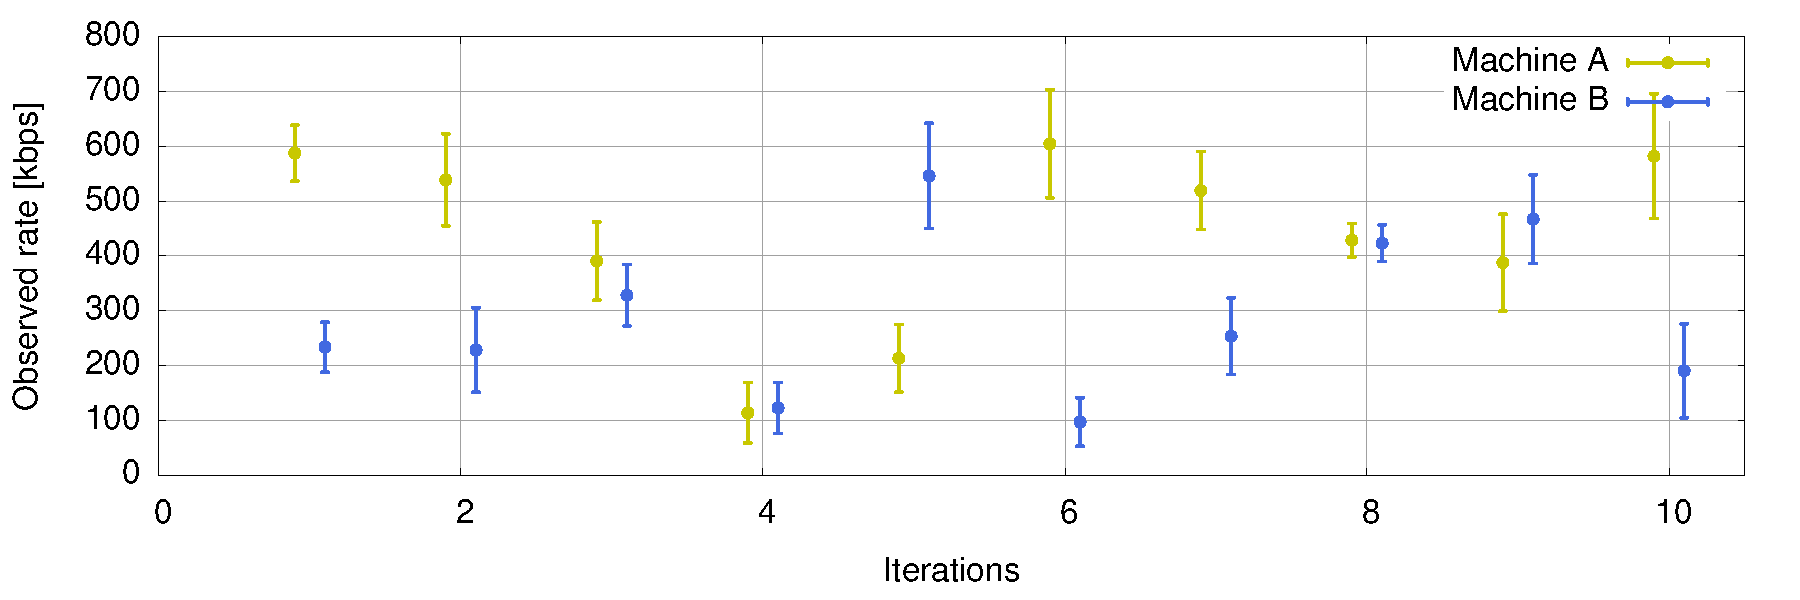
\includegraphics[width=\textwidth]{./figures/1mb_01s_mean_deviation_bw.pdf}
      \caption[1 Mbit/s and 100ms queue size]{1 Mbit/s and 100ms queue size.}
	\label{fig:1mb_01s_mean_deviation_bw}
        \end{subfigure}
        \caption{Bandwidth and mean for 1 Mbit/s with multiple queue sizes}
        \label{fig:1mb_mean_deviation_bw}
\end{figure}

\begin{figure}[htp]
        \centering
        \begin{subfigure}[h]{1\textwidth}
                \centering
                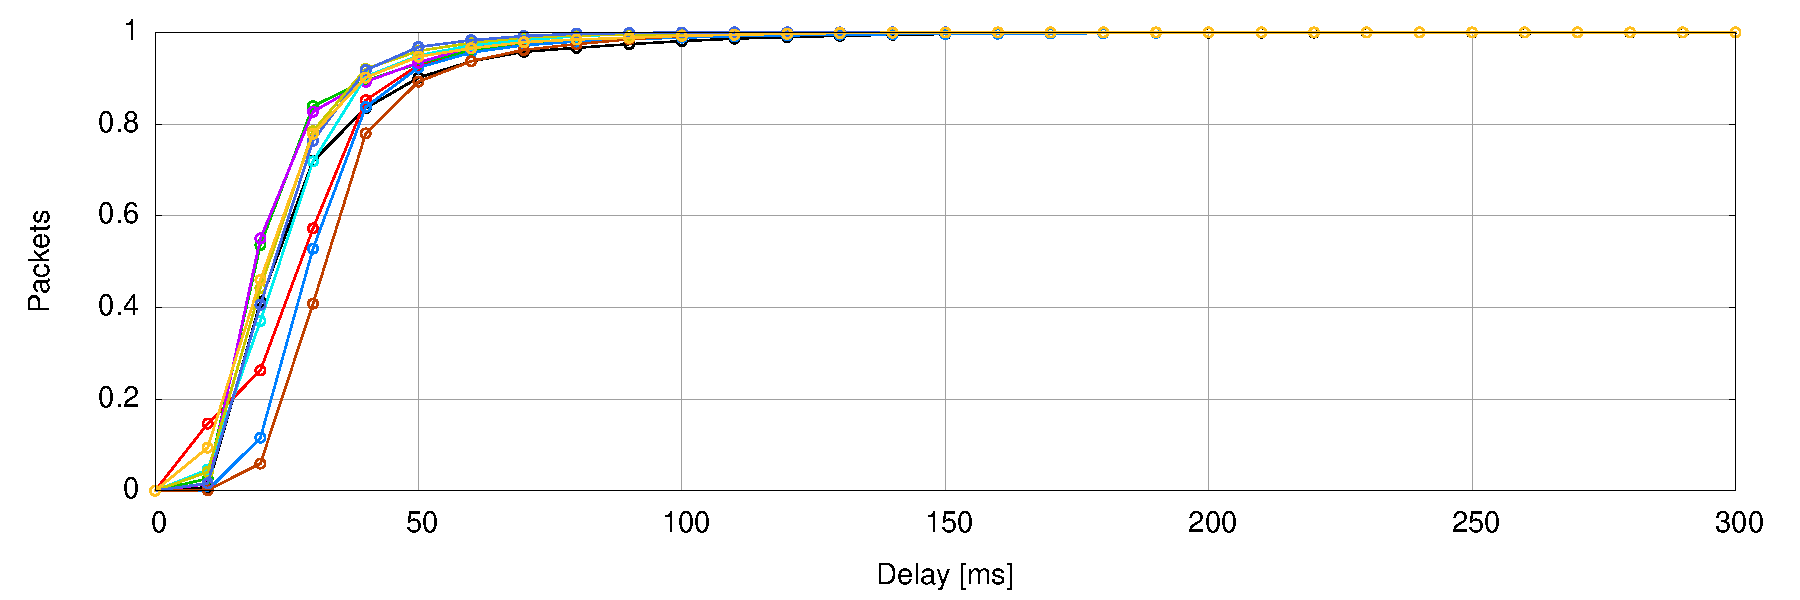
\includegraphics[width=\textwidth]{./figures/1mb_10s_total_delay_distribution.pdf}
      \caption[1 Mbit/s and 10s queue size]{1 Mbit/s and 10s queue size.}
	\label{fig:1mb_10s_total_delay_distribution}
        \end{subfigure}
        
        \begin{subfigure}[h]{1\textwidth}
                \centering
                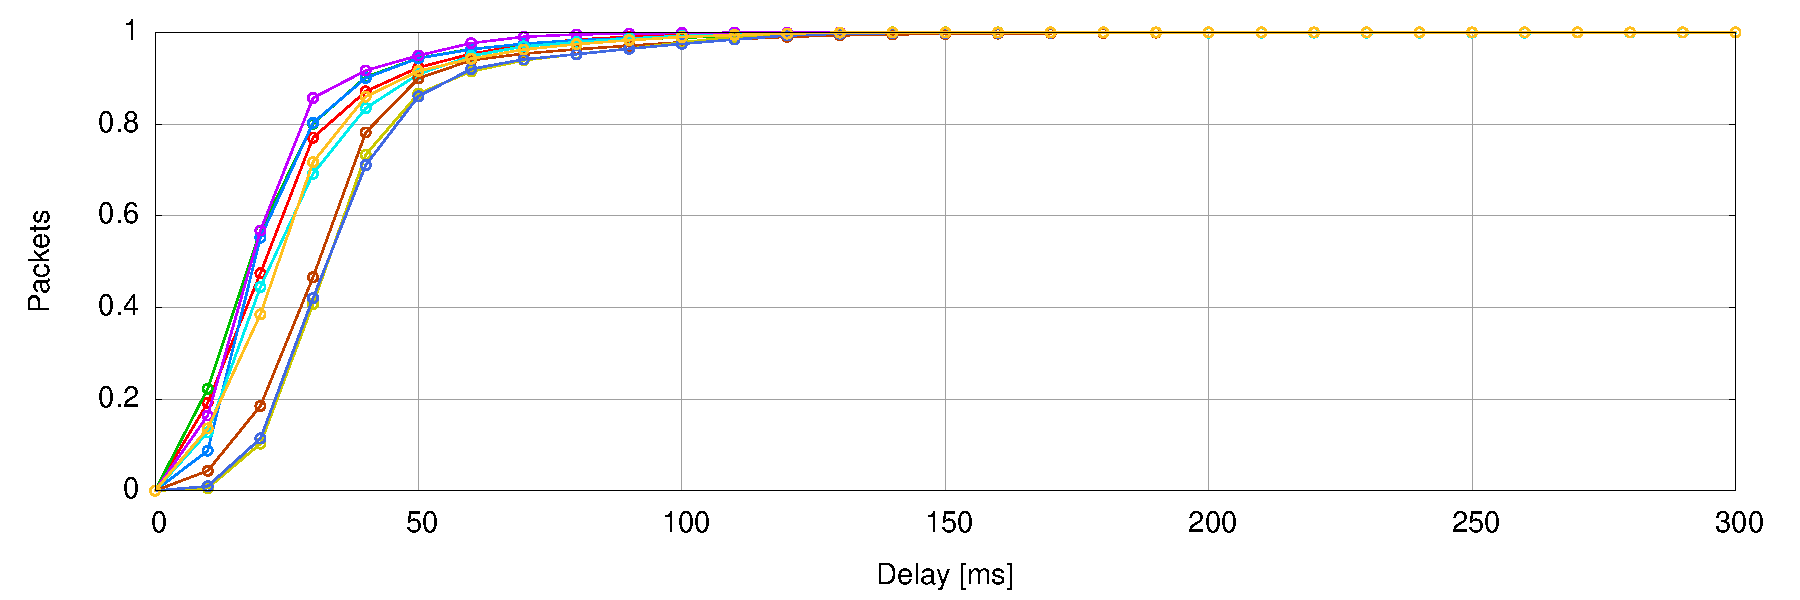
\includegraphics[width=\textwidth]{./figures/1mb_1s_total_delay_distribution.pdf}
      \caption[1 Mbit/s and 1s queue size]{1 Mbit/s and 1s queue size.}
	\label{fig:1mb_1s_total_delay_distribution}
        \end{subfigure}

        \begin{subfigure}[h]{1\textwidth}
                \centering
                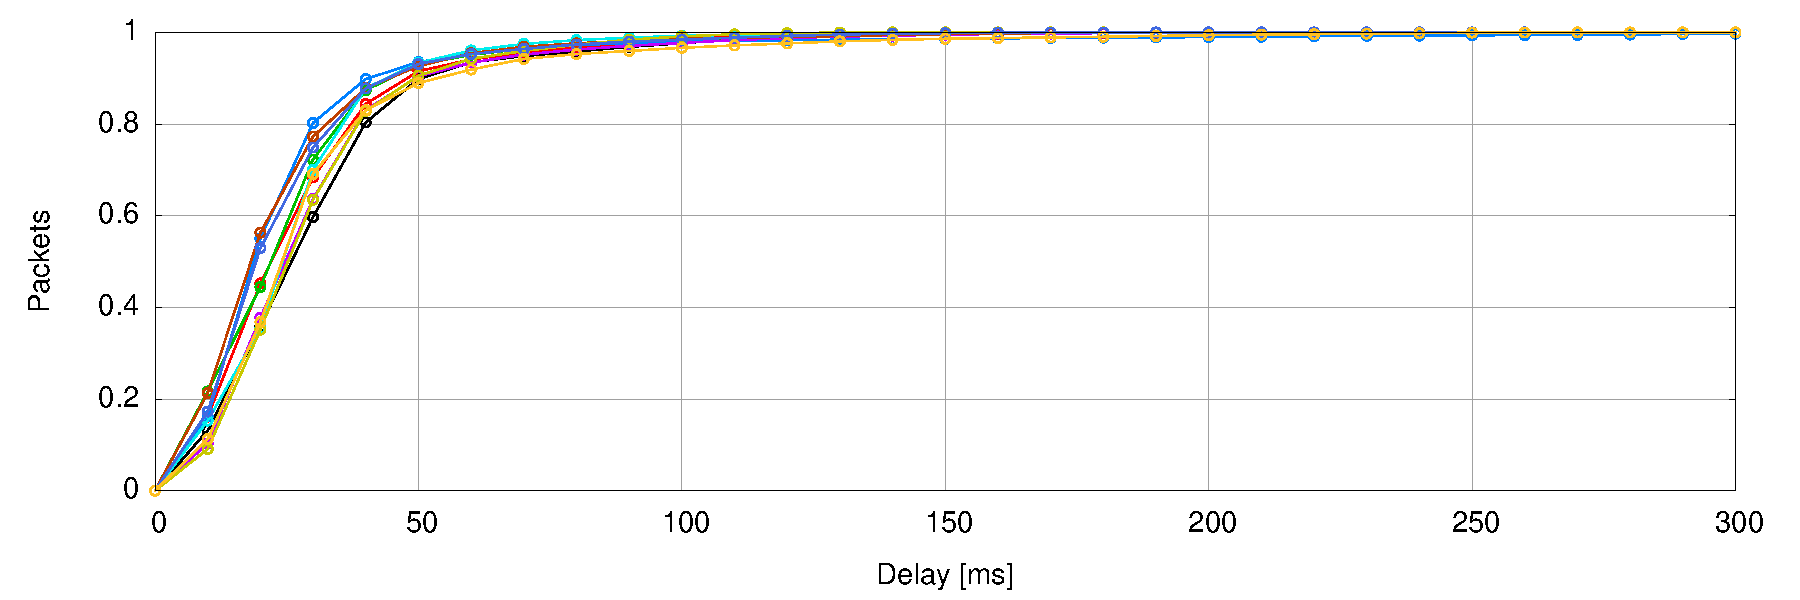
\includegraphics[width=\textwidth]{./figures/1mb_05s_total_delay_distribution.pdf}
      \caption[1 Mbit/s and 500ms queue size]{1 Mbit/s and 500ms queue size.}
	\label{fig:1mb_05s_total_delay_distribution}
        \end{subfigure}%
        
        \begin{subfigure}[h]{1\textwidth}
                \centering
                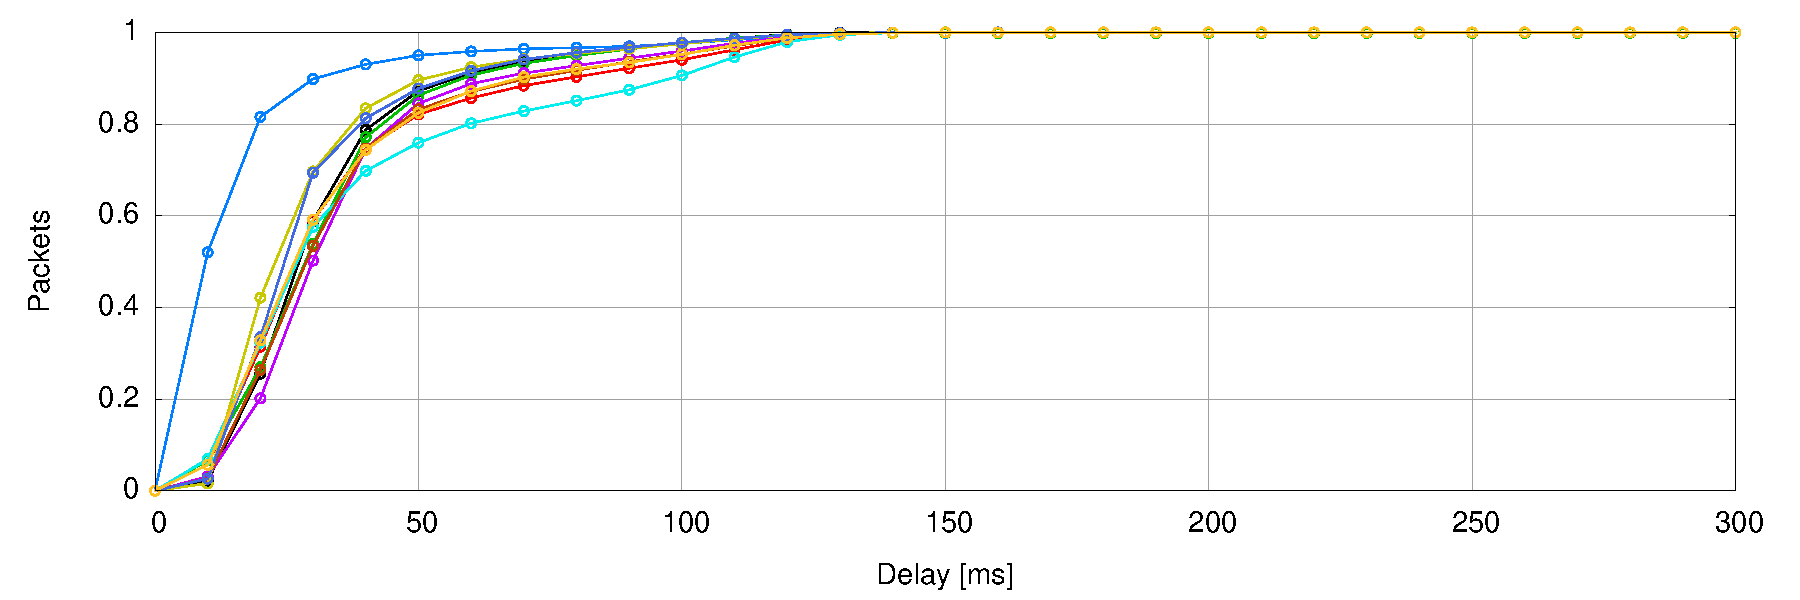
\includegraphics[width=\textwidth]{./figures/1mb_01s_total_delay_distribution.pdf}
      \caption[1 Mbit/s and 100ms queue size]{1 Mbit/s and 100ms queue size.}
	\label{fig:1mb_01s_total_delay_distribution}
        \end{subfigure}
        \caption{Delay distribution for 1 Mbit/s with multiple queue sizes}
        \label{fig:1mb_total_delay_distribution}
\end{figure}

\clearpage
\clearpage
\subsection{Loaded network}

Similar to the previous test, in this case we will be measuring the performance of WebRTC in a loaded network using a tool named {\it Iperf}. This tool will allow us to emulate traffic between our two peers loading the network according to our needs with UDP or TCP packets. The configuration we will use is the one shown in Figure~\ref{fig:iperfTest} with the clients running {\it Dummynet} instead of the relay. This scenario is chosen due its widely usage in real devices, having video calls meanwhile manipulating large amounts of online data is something that might happen when using WebRTC.

 \begin{figure}[h]
  \centering
    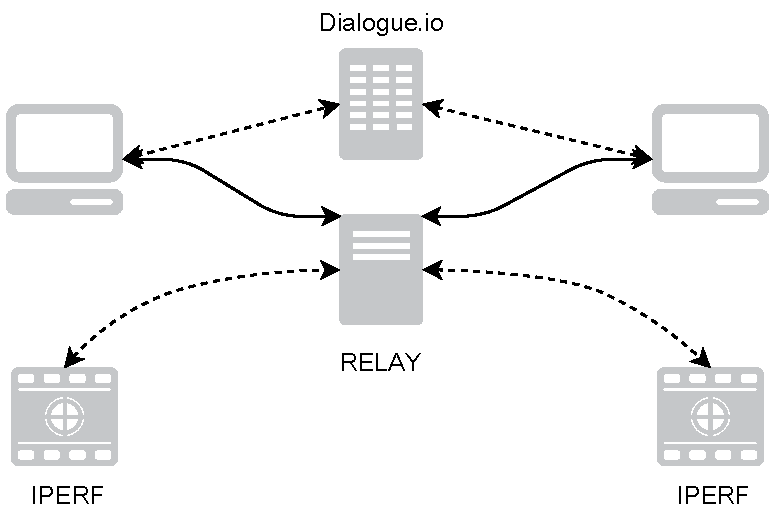
\includegraphics[width=0.8\textwidth]{./figures/IPERF.pdf}
      \caption[Topology for traffic flooded path using {\it Iperf}]{Topology for traffic flooded path using {\it Iperf}.}
	\label{fig:iperfTest}
\end{figure}

In this scenario we are interested in measuring also the behavior of real bandwidth setups for different environments, we will be testing the link with 100/10 Mbit/s and 20/4 Mbit/s limitations, the second one could be defined as the standard for HSPA networks. The data that will be sent to the other peer will be either 10 Mbit/s of TCP and UDP traffic or 2 Mbit/s.

First we will run the server as daemon on the recipient of the packets by executing:

\begin{verbatim}
# iperf -s -D
\end{verbatim}

The next step will rely on the usage of UDP or TCP, {\it Iperf} sends TCP packets by default, to do so we will run:

\begin{verbatim}
# iperf -c XXXX -t 300 {-u} -b 10m/2m 
\end{verbatim}

In the previous command, {\it -t} is the amount of time the test length, {\it -c} is the feature that configures the remote server to send the packets to, {\it -u} is going to be used to sent UDP datagrams instead of TCP and {\it -b} will define the amount of Mbit/s to be sent to the remote server. In this case every test is run three times.

Table~\ref{fig:tcp_iperf_no_dummynet} summarizes the results of the 10 Mbit/s TCP packet test without {\it Dummynet} constraints in the link.

\begin{table}[h]
\begin{center}
    \begin{tabular}{c D{,}{\pm}{-1} D{,}{\pm}{-1} D{,}{\pm}{-1} }
   	 \toprule
	\textit{}
	& \multicolumn{1}{c}{\textit{Machine A}}
	& \multicolumn{1}{c}{\textit{Machine B}}
	& \multicolumn{1}{c}{\textit{Overall}}\\
	\midrule
	\textbf{CPU (\%)} & 81.06 ,5.2 & 82.15 ,5.23 & 81.16 ,5.22\\
	\textbf{Memory (\%)} & 35.65 ,0.43 & 34.27 ,0.39 & 34.96 ,0.41\\
	\textbf{Bandwidth (Kbit/s)} & 990.11 ,202.62 & 1250.13 ,264.38 & 1120.12 ,233.506\\
	\textbf{Setup time (ms)} & 1533.66 ,11.3 & 1577.66 ,41.89 & 1555 ,32.59\\
	\textbf{RTT (ms)} & 25.61 ,16.02 & 24.76 ,14.11 & 25.19 ,15.07\\
	\textbf{Delay (ms)} & 81.61 ,11.42 & 83.99 ,11.42 & 81.61 ,11.42\\
	\bottomrule
    \end{tabular}
    \caption[IPERF 10 Mbit/s TCP test without link constraints]{IPERF 10 Mbit/s TCP test without link constraints.}
    \label{fig:tcp_iperf_no_dummynet}
\end{center}
\end{table}

The bandwidth rate in the call is affected by the traffic of TCP packets along the path, at the same time we are getting higher delays. Call behavior in this environment changes in every iteration being unpredictable, Figure~\ref{fig:iperfTestStd} represents the bandwidth mean and deviation of every iteration, we can easily observe that in the worst case we are getting three times less rate than the optimum case, ranging from 1.5 Mbit/s to under 400 Kbit/s in the worst iteration.

 \begin{figure}[h]
  \centering
    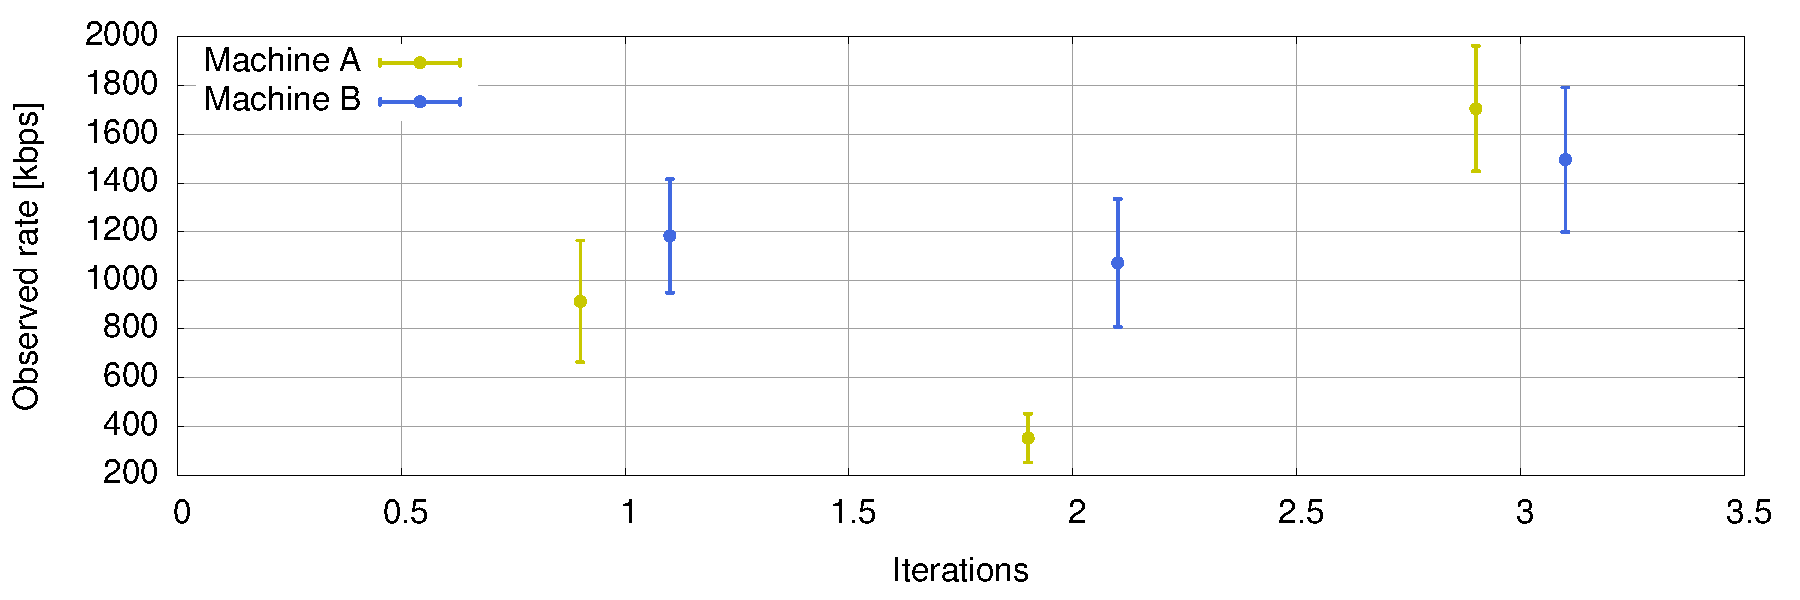
\includegraphics[width=1\textwidth]{./figures/iperf_std_mean_deviation_bw.pdf}
      \caption[Bandwidth mean and deviation for 10 Mbit/s TCP {\it Iperf} test without link constraints]{Bandwidth mean and deviation for 10 Mbit/s TCP {\it Iperf} test without link constraints.}
	\label{fig:iperfTestStd}
\end{figure}

We can observe some interesting behavior in all three iterations when looking at Figure~\ref{fig:iperfTestStdDelay} total delay distribution, the response varies from all three tests being all of them bad, a lot of sudden delay changes will appear during the call making real time communication difficult. The delay deviation is small but the tolerance for TCP flooded networks is low int WebRTC.

 \begin{figure}[h]
  \centering
    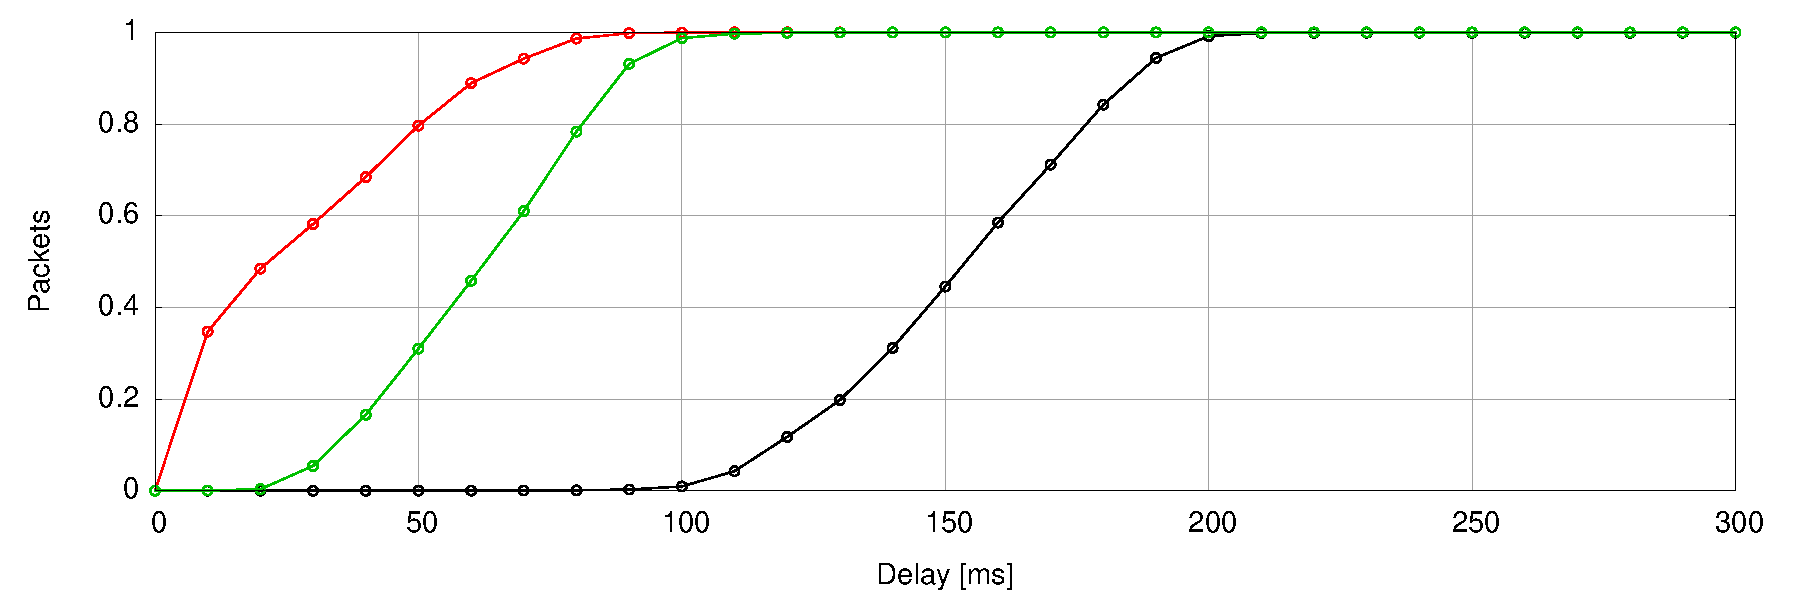
\includegraphics[width=1\textwidth]{./figures/iperf_std_total_delay_distribution.pdf}
      \caption[Total delay distribution for 10 Mbit/s TCP {\it Iperf} test without link constraints]{Total delay distribution for 10 Mbit/s TCP {\it Iperf} test without link constraints.}
	\label{fig:iperfTestStdDelay}
\end{figure}

Now we will test the behavior when sending those 10 Mbit/s with UDP and TCP in a constrained link of 100/10 (downlink/uplink), in this test {\it Dummynet} scripts have been executed on the client side instead of in the Relay. Table~\ref{fig:tcp_iperf_100in_10out} shows the different bandwidth responses between TCP and UDP traffic, in both cases the link constraint have been the same but the result varies. We will se an increase of rate with TCP flooded packets but also an increase of delay, this delay might be produced due the need of processing more packets with TCP than the simple mechanism of UDP.

\begin{table}[h]
\begin{center}
    \begin{tabular}{c D{,}{\pm}{-1} D{,}{\pm}{-1} D{,}{\pm}{-1} }
   	 \toprule
	\textit{}
	& \multicolumn{1}{c}{\textit{Machine A}}
	& \multicolumn{1}{c}{\textit{Machine B}}
	& \multicolumn{1}{c}{\textit{Overall}}\\
	\midrule
	\textbf{Bandwidth UDP (Kbit/s)} & 159.41 ,28.69 & 149.04 ,25.76 & 159.23 ,27.23 \\
	\textbf{Delay UDP (ms)} & 98.07 ,3.14 & 98.85 ,2.75 & 96.85 ,2.94 \\
	\hline
	\hline
	\textbf{Bandwidth TCP (Kbit/s)} & 208.97 ,20.64 & 194.41 ,18.9 & 201.69 ,19.77\\
	\textbf{Delay TCP (ms)} & 146.9 ,4.38 & 147.92 ,4 & 147.41 ,4.23 \\
	\bottomrule
    \end{tabular}
    \caption[IPERF 10 Mbit/s TCP and UDP test with constrained 100/10 Mbit/s link]{IPERF 10 Mbit/s TCP and UDP test with constrained 100/10 Mbit/s link.}
    \label{fig:tcp_iperf_100in_10out}
\end{center}
\end{table}

Delay distribution response in a constrained environment (Figure~\ref{fig:10m_udp_total_delay_distribution} and \ref{fig:10m_tcp_total_delay_distribution}) is smoother compared to Figure~\ref{fig:iperfTestStdDelay}, the absolute amount of delay is larger but the distribution curve is better for WebRTC needs as it does not have any sudden increase of delay. Delay response when having constraints will output a better delay distribution but with higher RTT in the link.

\begin{figure}
        \centering
        \begin{subfigure}[b]{0.5\textwidth}
                \centering
                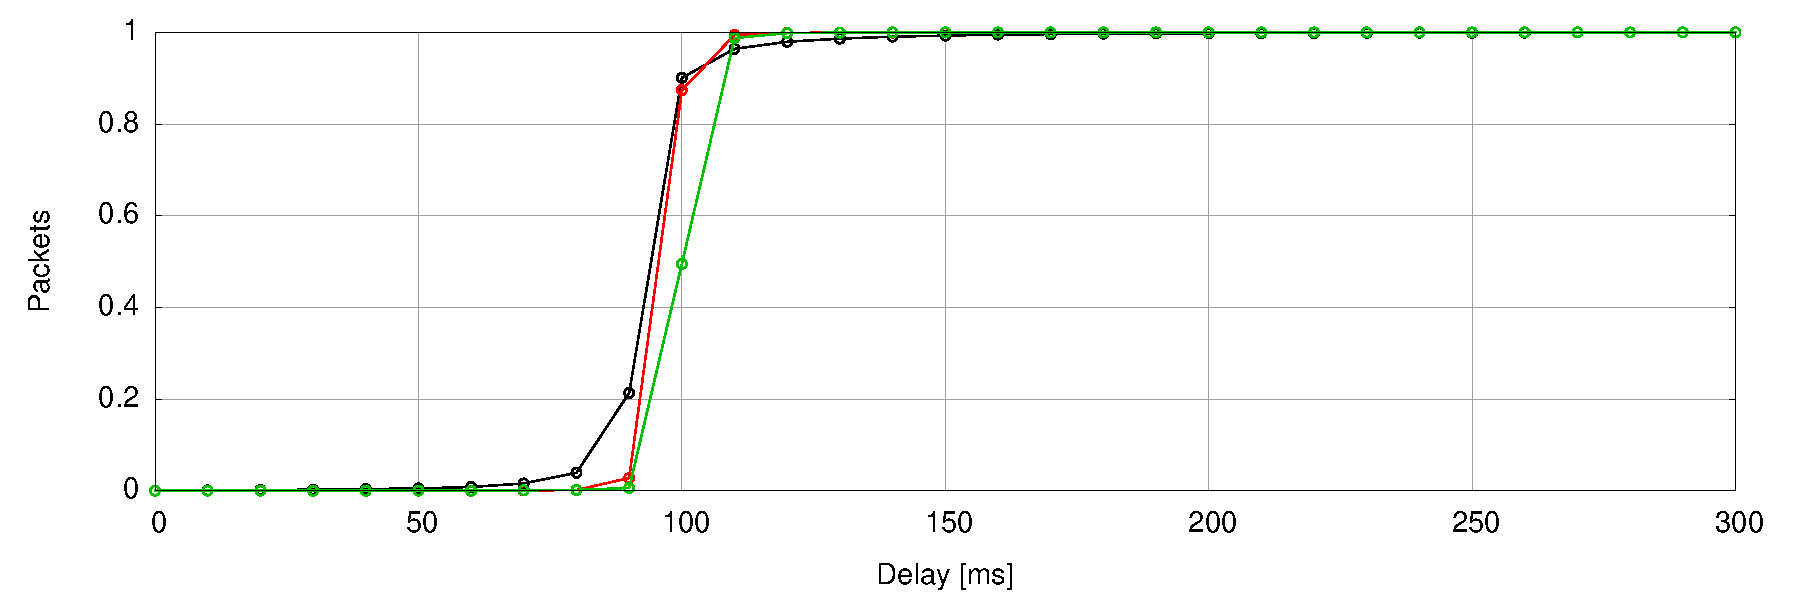
\includegraphics[width=\textwidth]{./figures/10m_udp_total_delay_distribution.pdf}
                \caption{Delay distribution response for UDP test}
                \label{fig:10m_udp_total_delay_distribution}
        \end{subfigure}%
        ~ %add desired spacing between images, e. g. ~, \quad, \qquad etc.
          %(or a blank line to force the subfigure onto a new line)
        \begin{subfigure}[b]{0.5\textwidth}
                \centering
                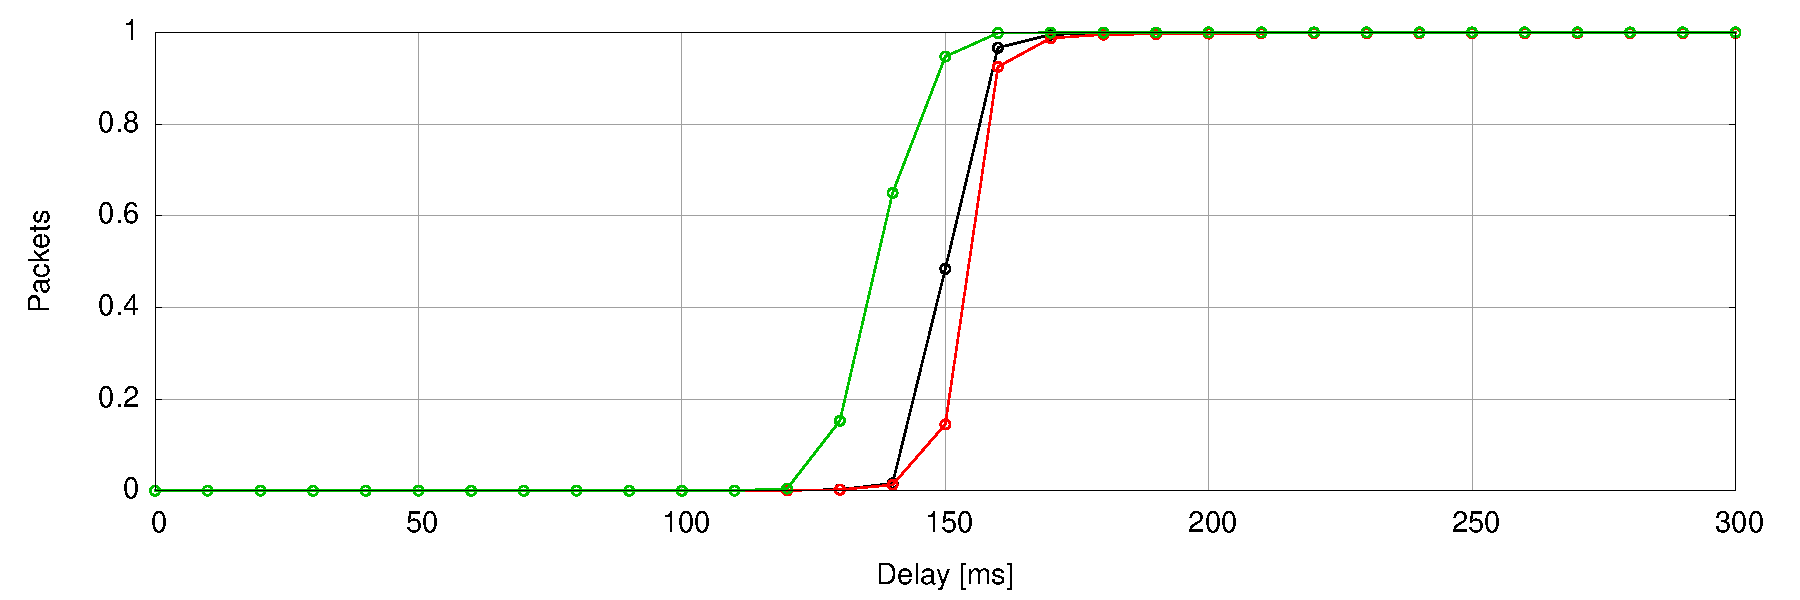
\includegraphics[width=\textwidth]{./figures/10m_tcp_total_delay_distribution.pdf}
                \caption{Delay distribution response for TCP test}
                \label{fig:10m_tcp_total_delay_distribution}
        \end{subfigure}
        \caption[10 Mbit/s UDP/TCP {\it Iperf} test with 100/10 link condition]{10 Mbit/s UDP/TCP {\it Iperf} test with 100/10 link condition.}
        \label{fig:10m_tcp_udp_distribution}
\end{figure}

When testing the 2 Mbit/s TCP and UDP flows with 20/4 Mbit/s constraints results are surprisingly close to the version without constraints, we are testing this configuration due to its similitudes to HSDPA networks that carry a similar averaged bandwidth. Unstable bandwidth is also noticed in this test but values for the rate are much higher and delay distribution graphs are similar to Figure~\ref{fig:10m_tcp_udp_distribution}. We are using 2 Mbit/s flows to imitate the encoding rate for an online streaming 1280x720 HD video.\footnote{http://www.adobe.com/devnet/adobe-media-server/articles/dynstream_live/popup.html}

Table~\ref{fig:tcp_iperf_20in_4out} describes the output we had in terms of rate and delay for the 2 Mbit/s test in a HSDPA type network. Rate adaptation is good even having an small uplink capacity of 4 Mbit/s, the way the rate is adapted to this link confirms that in this kind of not delayed or lossy low latency networks WebRTC could perform properly with simultaneous ongoing traffic. 

\begin{table}[h]
\begin{center}
    \begin{tabular}{c D{,}{\pm}{-1} D{,}{\pm}{-1} D{,}{\pm}{-1} }
   	 \toprule
	\textit{}
	& \multicolumn{1}{c}{\textit{Machine A}}
	& \multicolumn{1}{c}{\textit{Machine B}}
	& \multicolumn{1}{c}{\textit{Overall}}\\
	\midrule
	\textbf{Bandwidth UDP (Kbit/s)} & 683.81 ,259.38 & 749.66 ,249.69 & 716.74 ,254.53 \\
	\textbf{Delay UDP (ms)} & 56.34 ,2.83 & 54.31 ,2.64 & 55.32 ,2.74 \\
	\hline
	\hline
	\textbf{Bandwidth TCP (Kbit/s)} & 760.94 ,238.44 & 1174.95 ,235.12 & 967.94 ,236.78\\
	\textbf{Delay TCP (ms)} & 85.18 ,2.3 & 80.04 ,2.26 & 82.61 ,2.28 \\
	\bottomrule
    \end{tabular}
    \caption[IPERF 2 Mbit/s TCP and UDP test with constrained 20/4 Mbit/s link]{IPERF 2 Mbit/s TCP and UDP test with constrained 20/4 Mbit/s link.}
    \label{fig:tcp_iperf_20in_4out}
\end{center}
\end{table}

From the delay distribution point of view (Figure~\ref{fig:2m_tcp_udp_distribution}), the output is similar in both tests being TCP slightly better (\ref{fig:2m_tcp_total_delay_distribution}) with less absolute delay and with an acceptable variation.

\begin{figure}[h]
        \centering
        \begin{subfigure}[b]{0.5\textwidth}
                \centering
                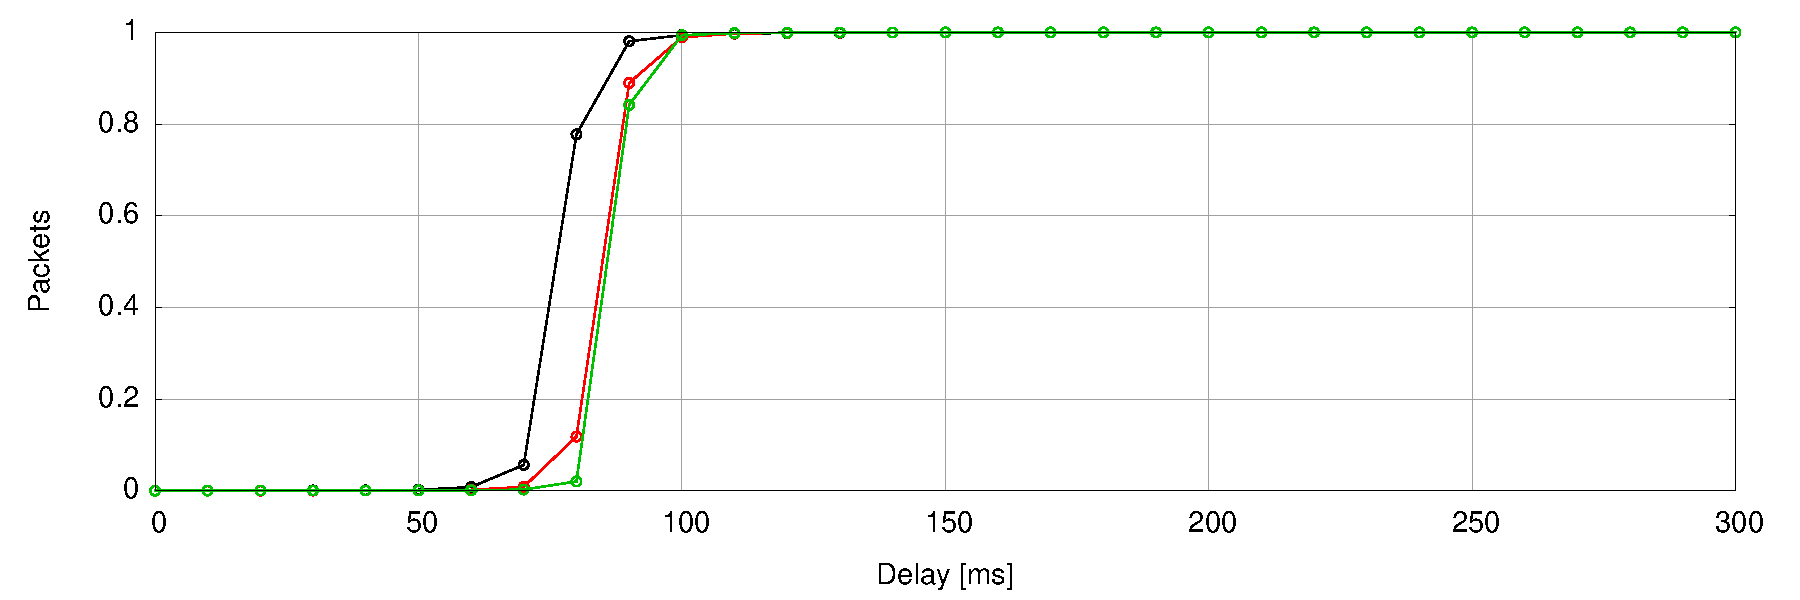
\includegraphics[width=\textwidth]{./figures/2m_udp_total_delay_distribution.pdf}
                \caption{Delay distribution response for UDP test}
                \label{fig:2m_udp_total_delay_distribution}
        \end{subfigure}%
        ~ %add desired spacing between images, e. g. ~, \quad, \qquad etc.
          %(or a blank line to force the subfigure onto a new line)
        \begin{subfigure}[b]{0.5\textwidth}
                \centering
                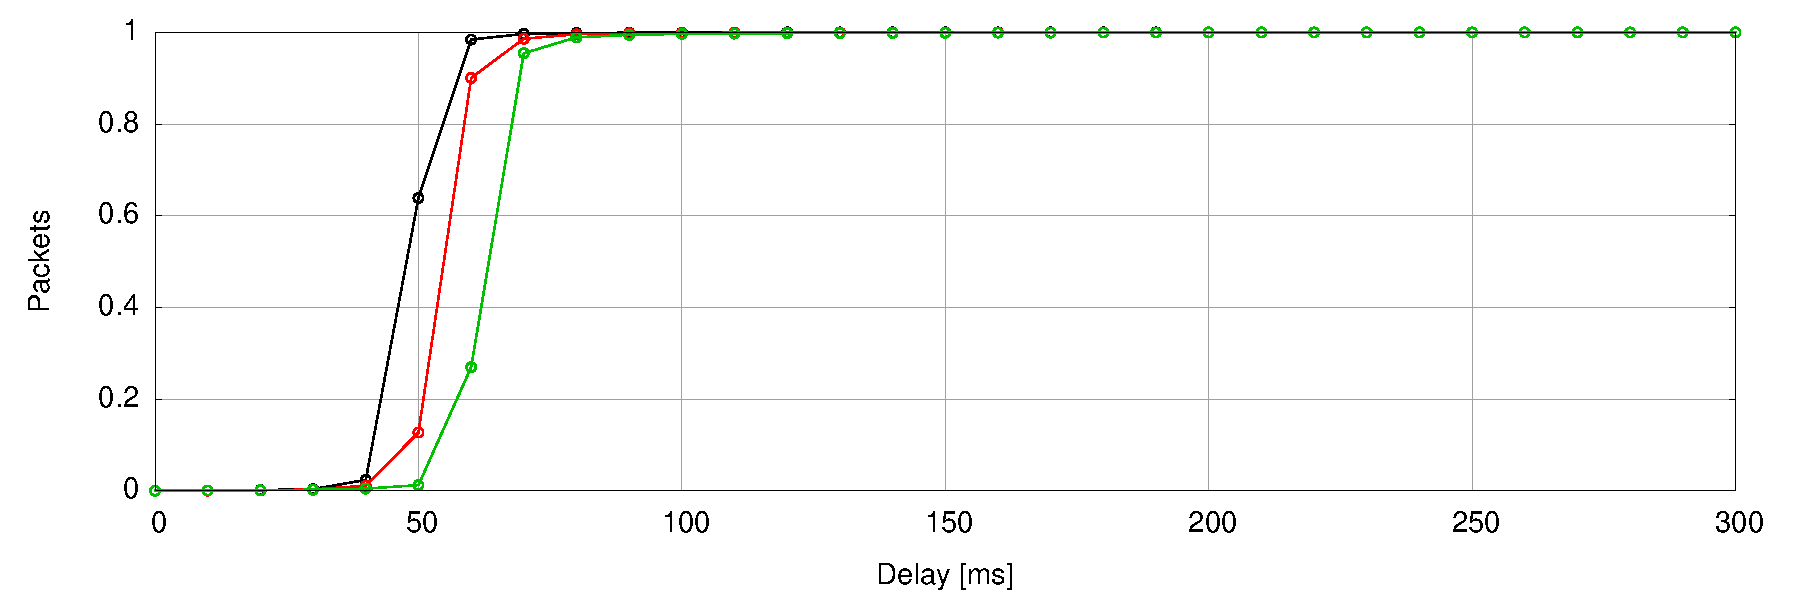
\includegraphics[width=\textwidth]{./figures/2m_tcp_total_delay_distribution.pdf}
                \caption{Delay distribution response for TCP test}
                \label{fig:2m_tcp_total_delay_distribution}
        \end{subfigure}
        \caption[2 Mbit/s UDP and TCP {\it Iperf} test with 20/4 link condition]{2 Mbit/s UDP and TCP {\it Iperf} test with 20/4 link condition.}
        \label{fig:2m_tcp_udp_distribution}
\end{figure}

In general, the response of WebRTC congestion mechanisms with ongoing link traffic should be better as this environment will be common for all users. The bandwidth mechanism produces an acceptable call rate but should produce delays smaller than one second which are acceptable from the usability perspective, the delay distribution for the standard case with an ongoing traffic of 10 Mbit/s is not as good as expected but it might be due to the high capacity on the path and the way {\it Iperf} simulates the traffic.

\subsection{Parallel calls}

In this part of the test we will be checking how WebRTC handles multiple parallel calls with different peers, this is not to me mixed with mesh style of topology as it will be running using different tabs or processes through the same TURN path. Figure~\ref{fig:parallelCalls} represents the topology used for the test.

 \begin{figure}[h]
  \centering
    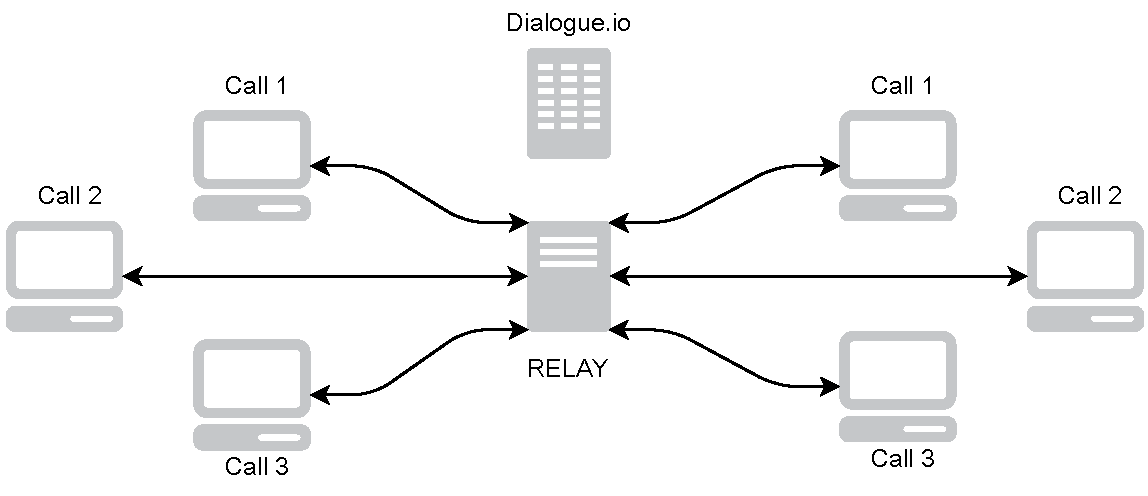
\includegraphics[width=1\textwidth]{./figures/ParallelCalls.pdf}
      \caption[Topology for three different parallel calls using the same link]{Topology for three different parallel calls using the same link.}
	\label{fig:parallelCalls}
\end{figure}

We will run a combined batch of tests using 2 and 3 simultaneous calls without {\it Dummynet} or with 20 Mbit/s and 10 Mbit/s bandwidth limitation for the link. The case without any constraint will run with the standard 100 Mbit/s of the ethernet link capacity. For the test we have focused in running the calls in the same machine but in different processes.

This kind of environment will be given in local networks or it could be compared with mesh topologies handling multiple peer connections, from the resources perspective it will be interesting to observe the CPU and memory consumption as every PeerConnection will be working in a different process, the machine used carries 1 CPU and 2 Gb of RAM.

\begin{table}[h]
\begin{center}
    \begin{tabular}{c D{,}{\pm}{-1} D{,}{\pm}{-1} D{,}{\pm}{-1} }
   	 \toprule
	\textit{}
	& \multicolumn{1}{c}{\textit{CPU (\%)}}
	& \multicolumn{1}{c}{\textit{Memory (\%)}}\\
	\midrule
	\textbf{Three calls} & 99.25 ,2.41 & 44.99 ,0.5 \\
	\textbf{Two calls 20 Mbit/s} & 95.67 ,3.51 & 46.16 ,0.37 \\
	\textbf{Two calls 10 Mbit/s} & 86.83 ,5.03 & 44.91 ,0.32 \\
	\textbf{Two calls} & 81.6 ,6.48 & 42.61 ,0.35 \\
	\bottomrule
    \end{tabular}
    \caption[Memory and CPU consumption rates for parallel calls in different link conditions]{Memory and CPU consumption rates for parallel calls in different link conditions.}
    \label{fig:cpu_mem_parallel}
\end{center}
\end{table}

Table~\ref{fig:cpu_mem_parallel} describes the resource comparison between two and three simultaneous calls. CPU usage is critical when handling three peer connections or when the network condition forces the congestion mechanism to continuously adapt the bandwidth and encoding. In this test, each call is placed in a different process which should improve the results as the OS will handle them better than in a single thread. When the CPU load gets to its maximum the performance of WebRTC for encoding/decoding and transmission is deprecated, in this kind of topologies having high CPU performance increases the call quality.

\begin{table}[h]
\begin{center}
    \begin{tabular}{c D{,}{\pm}{-1} D{,}{\pm}{-1} D{,}{\pm}{-1} }
   	 \toprule
	\textit{}
	& \multicolumn{1}{c}{\textit{Machine A}}
	& \multicolumn{1}{c}{\textit{Machine B}}
	& \multicolumn{1}{c}{\textit{Overall}}\\
	\midrule
	\textbf{Three calls} & 768.04 ,180.93 & 850.1 ,223.84 & 809.07 ,202.38 \\
	\textbf{Two calls 20 Mbit/s} & 432.56 ,141.32 & 531.13 ,169.82 & 481.85 ,155.56 \\
	\textbf{Two calls 10 Mbit/s} & 178.83 ,60.05 & 141.83 ,42.02 & 160.24 ,51.04 \\
	\textbf{Two calls} & 392.08 ,181.9 & 545.94 ,259.27 & 469.01 ,221.09 \\
	\bottomrule
    \end{tabular}
    \caption[Bandwidth rates for parallel calls in different link conditions]{Bandwidth rates for parallel calls in different link conditions.}
    \label{fig:bw_parallel}
\end{center}
\end{table}

The bandwidth represented in Table~\ref{fig:bw_parallel} is the one used per each machine with the calls together, we will study the worst case. The bandwidth for three calls is to use an average of 800 Kbit/s with different responses in every case, the deviation is approximately $\pm202$ Kbit/s. 

\begin{figure}[h]
  \centering
    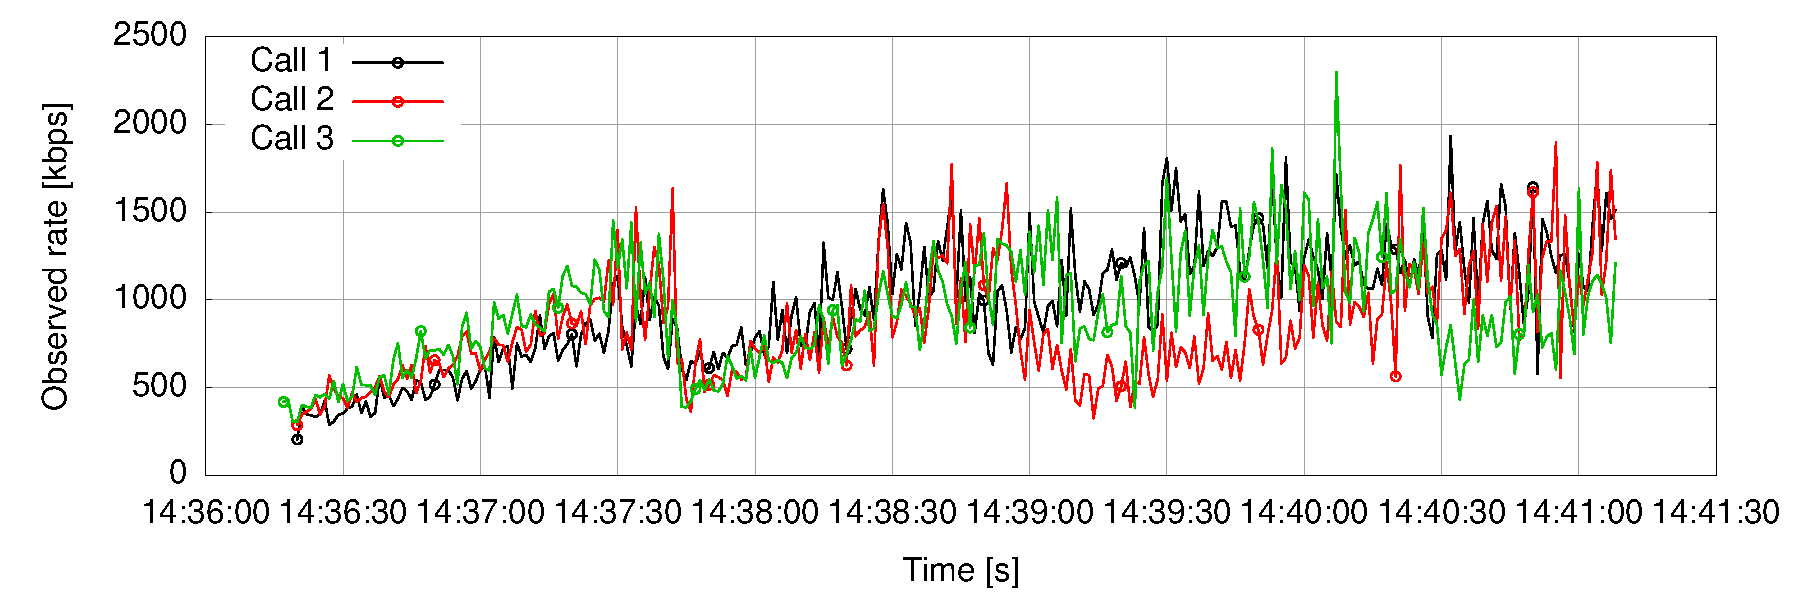
\includegraphics[width=1\textwidth]{./figures/sync_three-calls.pdf}
      \caption[Bandwidth representation for all remote streams in a synchronous three peer parallel call for first iteration]{Bandwidth representation for all remote streams in a synchronous three peer parallel call for first iteration.}
	\label{fig:three_parallel}
\end{figure}


Furthermore, it is interesting to see the global rate on the call as the bandwidth averaged is not following a stable value, Figure~\ref{fig:three_parallel} represents the bandwidth during all call for the remote video stream of the three peers. We can see how the rate mechanism tries to use the maximum available rate for the actual video encoding but fails to reach the 2 Mbit/s as multiple calls are running and behaving in the same way, this decision is taken also considering the delay that limits the maximum available rate for the call. Figure represents the delay on the same streams during the call, we can observe those peaks of delay during the same period as the bandwidth rise, the result of this is the sudden drop of bandwidth, this mechanism is triggered multiple times.

\begin{figure}[h]
        \centering
        \begin{subfigure}[b]{0.5\textwidth}
                \centering
                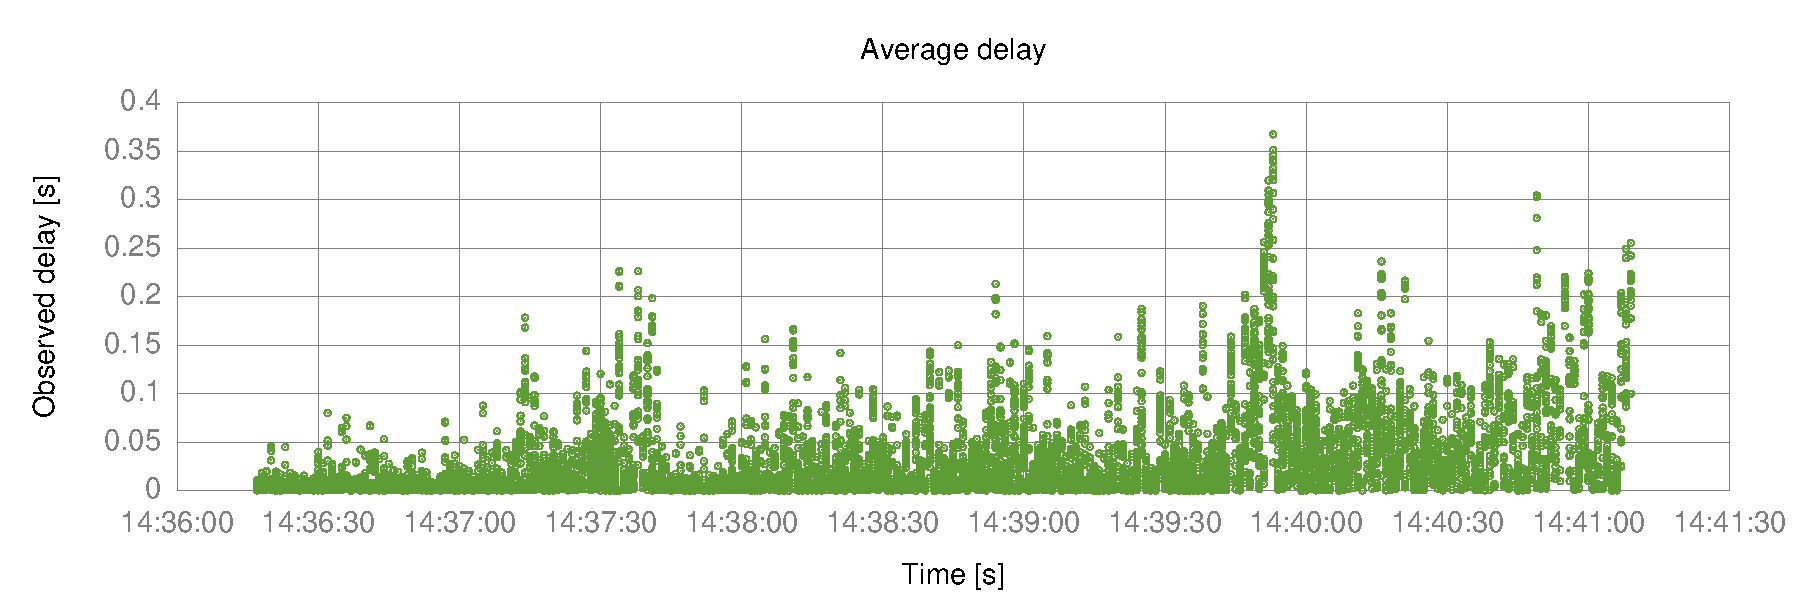
\includegraphics[width=\textwidth]{./figures/delay_three_parallel_1.pdf}
                \caption{Remote stream for call 1}
                \label{fig:three_parallel_1}
        \end{subfigure}%
        ~ %add desired spacing between images, e. g. ~, \quad, \qquad etc.
          %(or a blank line to force the subfigure onto a new line)
        \begin{subfigure}[b]{0.5\textwidth}
                \centering
                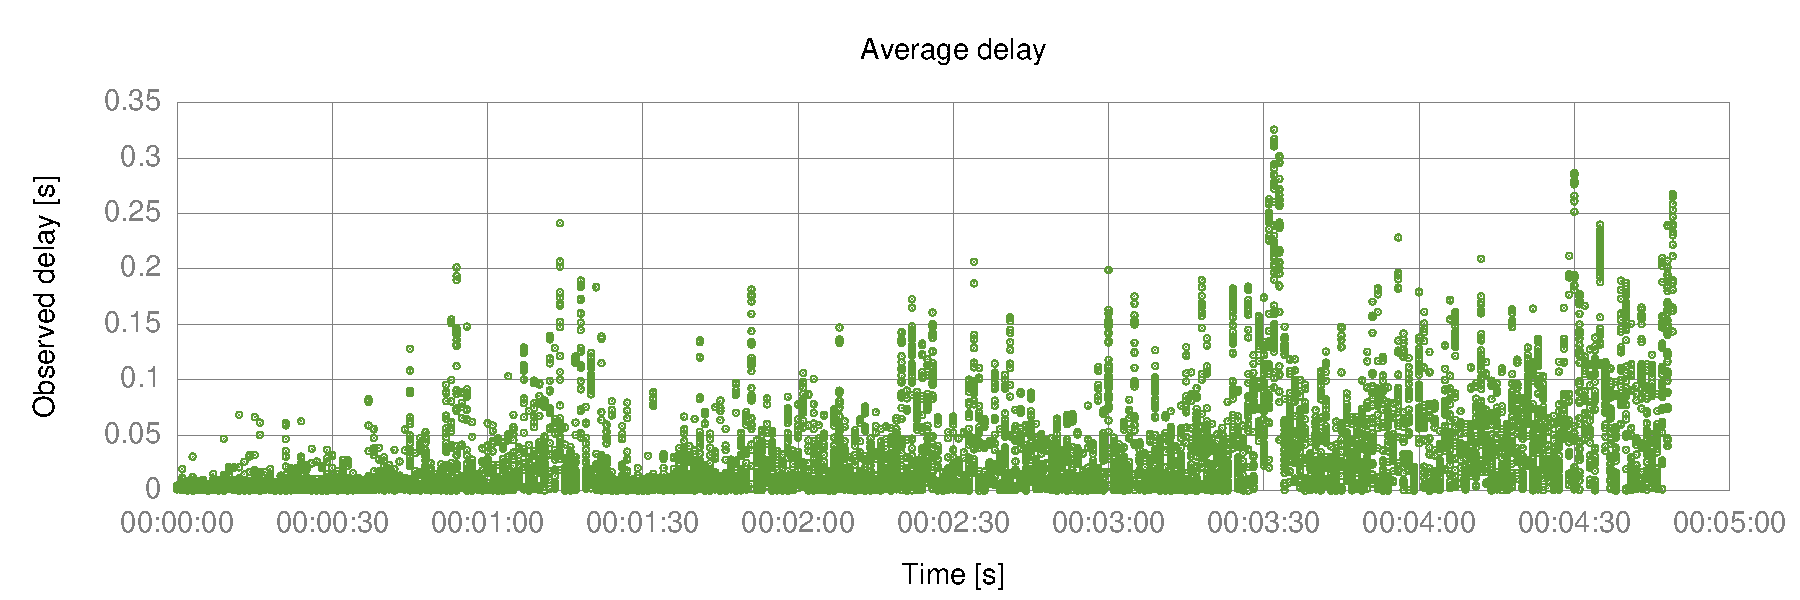
\includegraphics[width=\textwidth]{./figures/delay_three_parallel_2.pdf}
                \caption{Remote stream for call 2}
                \label{fig:three_parallel_2}
        \end{subfigure}        
        ~ %add desired spacing between images, e. g. ~, \quad, \qquad etc.
          %(or a blank line to force the subfigure onto a new line)
        \begin{subfigure}[b]{0.5\textwidth}
                \centering
                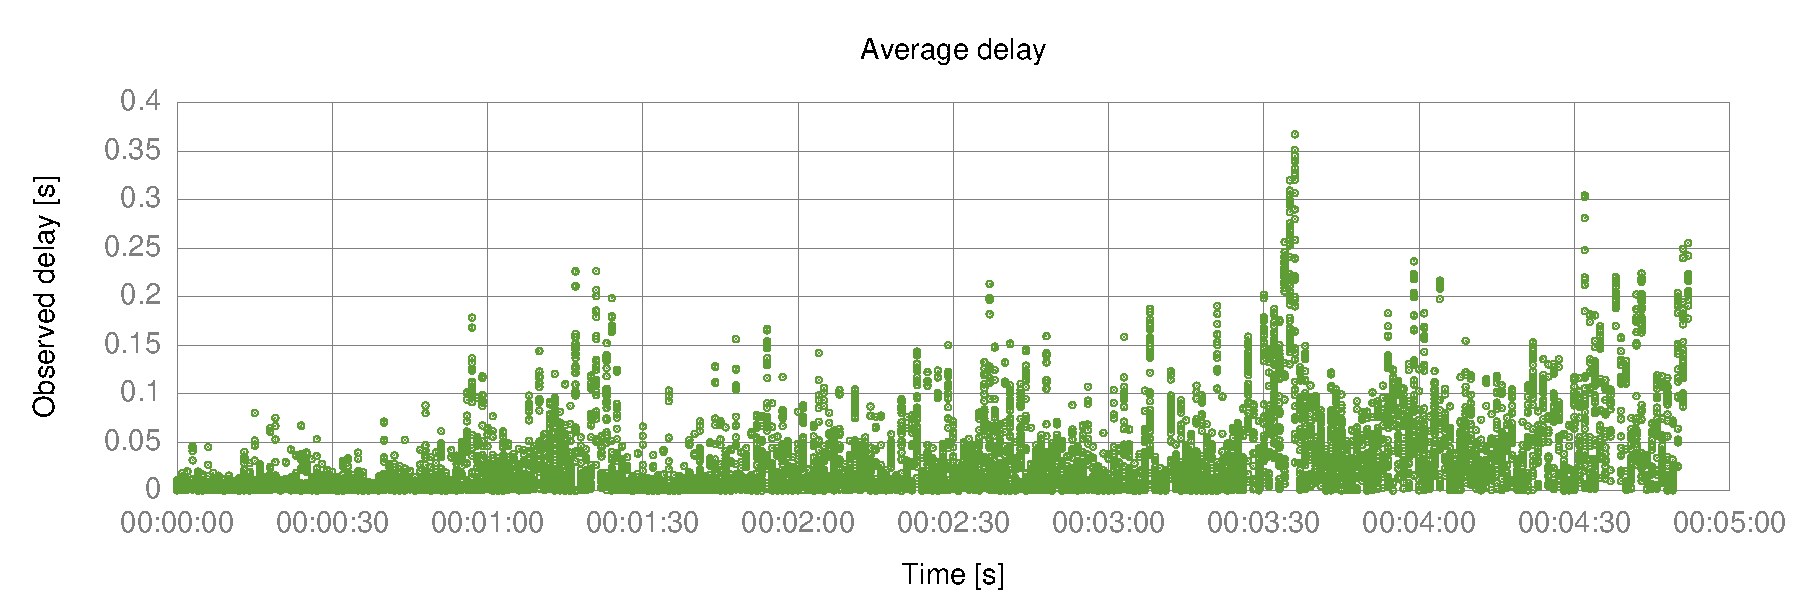
\includegraphics[width=\textwidth]{./figures/delay_three_parallel_3.pdf}
                \caption{Remote stream for call 3}
                \label{fig:three_parallel_3}
        \end{subfigure}
        \caption[Delay representation for all remote streams in a three peer parallel call]{Delay representation for all remote streams in a three peer parallel call.}
        \label{fig:delay_three_parallel}
\end{figure}

We can compare this scenario with the one in Figure~\ref{fig:1cd81aa8-bw}, the difference relays in the channel condition, in the example of Figure~\ref{fig:1cd81aa8-bw} the channel condition set high restrictions on the path making the rate drop and keep stable as the condition didn't change after that moment. In Figure~\ref{fig:delay_three_parallel}, path condition changes after the drop as it becomes available again as all the three peer calls behaved the same way. 

In general the delay response in all the calls is bad, Figure~\ref{fig:delayThreeCalls} plots the delay distribution of the three simultaneous calls, the slow increase of delay makes the call lag large and variable, probably the user experience for all the three calls will be bad.

\begin{figure}[h]
  \centering
    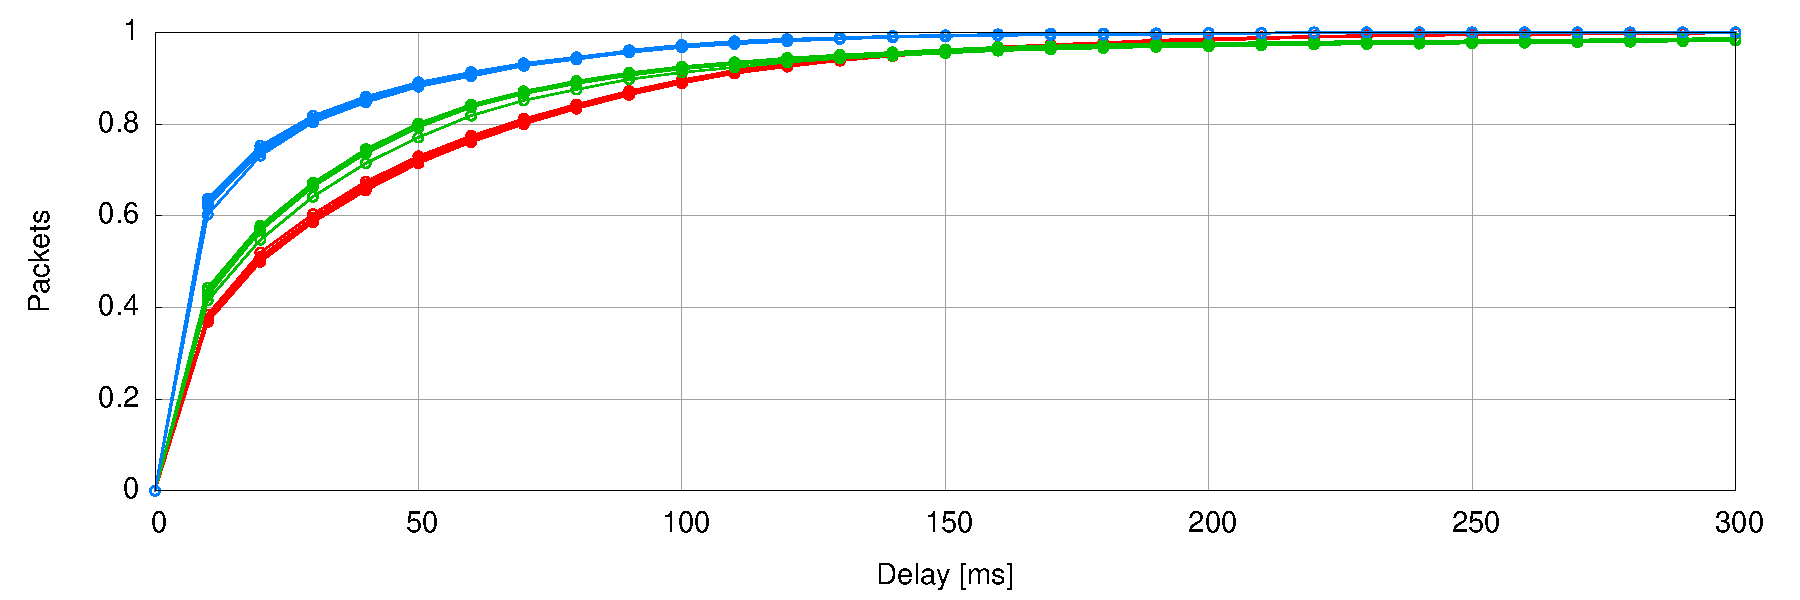
\includegraphics[width=1\textwidth]{./figures/three_parallel_total_delay_distribution.pdf}
      \caption[Total delay distribution for three parallel calls]{Total delay distribution for three parallel calls.}
	\label{fig:delayThreeCalls}
\end{figure}

The problem relies on the separate treatment of every peer connection, they have no acknowledge of having different similar processes going so the rate change cannot be constrained by the other ongoing calls. Notice that for this test all calls started at the same time, for this purpose we ran a second set of tests starting every call delayed by 15 seconds to check the behavior of the system.

After analyzing the captures of the new asynchronous call we can plot the averaged bandwidth to be approximately 1154 Kbit/s with $\pm250$ Kbit/s of deviation. Overall averaged results are significantly higher than in the previous case but we should have a close look at Figure that represents the bandwidth behavior of the three calls during all the duration for the first iteration we can observe that the average is high but one of the calls rate is very low.

\begin{figure}[h]
  \centering
    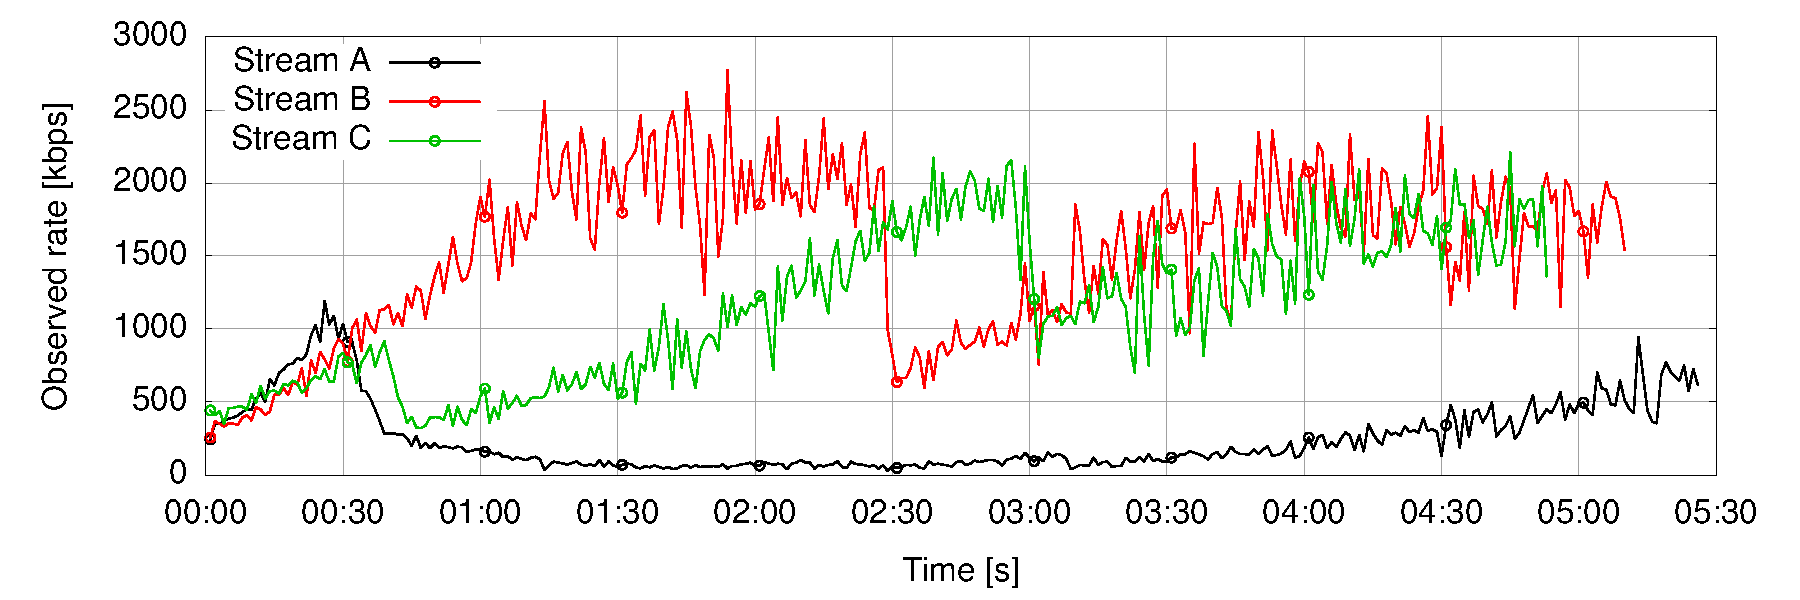
\includegraphics[width=1\textwidth]{./figures/async_three-calls.pdf}
      \caption[Bandwidth representation for all remote streams in an asynchronous three peer parallel call for iteration one]{Bandwidth representation for all remote streams in an asynchronous three peer parallel call for iteration one.}
	\label{fig:three_parallel}
\end{figure}

In this case, the first call that started to increase its rate suddenly drops it to approximately 100 Kbit/s and stays there along the call meanwhile the other two parallel calls try to obtain the maximum available bandwidth of the path. This environment is more approximated to the a real scenario as users won't start calls exactly at the same time but they will probably do that randomly, some calls quality will be degraded with barely no quality and others will have sudden drop of bandwidth affecting the interaction with the user.

\begin{figure}[h]
  \centering
    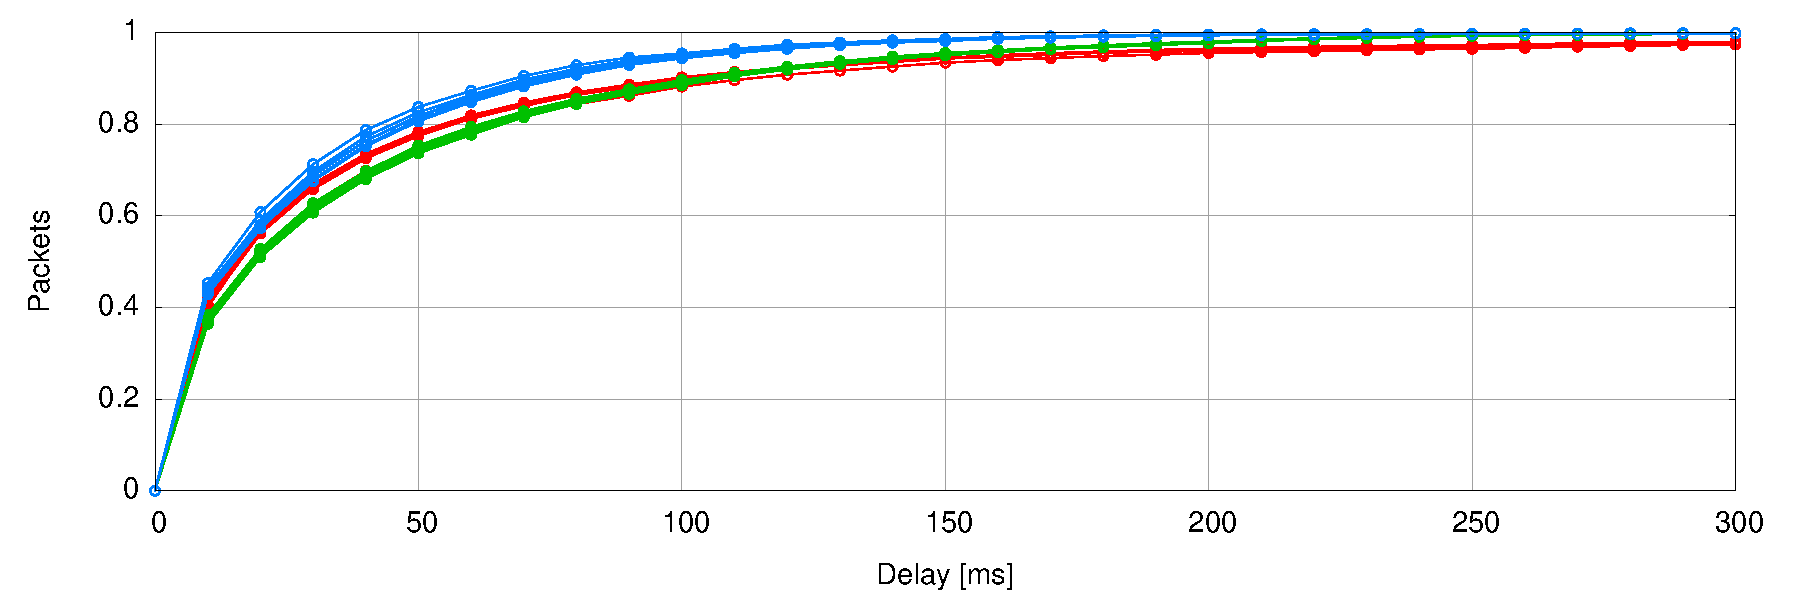
\includegraphics[width=1\textwidth]{./figures/async_total_delay_distribution.pdf}
      \caption[Total delay distribution for three asynchronous parallel calls]{Total delay distribution for three asynchronous parallel calls.}
	\label{fig:delayThreeCallsAsync}
\end{figure}

Figure~\ref{fig:delayThreeCallsAsync} represents the delay distribution for the asynchronous test, similar to the previous example (Figure~\ref{fig:delayThreeCalls}) but with a worst delay response. Delay will affect to the user experience having sudden cuts of communications of milliseconds that will occur randomly, they are not large but they are random and unexpected.

WebRTC should be able to identify parallel connections of the same type and balance the bandwidth usage, this is difficult as the transport level uses already existing RTP technology over UDP, the conclusion is that WebRTC will not be reliable for multiple parallel calls in an average computer.

\subsection{Mesh topology}

A common setup in real-time communications is video conferencing, this way of calling people is widely used in virtual meetings. Until this moment there were multiple available options in the market, with the arrival of WebRTC this feature extends to the web application world, with multiple options and features to be enabled with it. We will try to determine if WebRTC is mature enough to handle multiple peers at the same time and session, the way this is done varies depending on the technology, we will study pure peer-to-peer mesh networks.

The most common option for this kind of environments is to use an MCU to perform the relying of the media through a unique connection by multiplexing the streams in a single one. There are some MCU available in the market for WebRTC but the API is still not evolved enough to allow multiplexing of streams over the same Peer Connection, in the following updates of the API this should be enabled allowing developers to perform real media multiplexing. Some vendors offer MCUs that require extra plugins to be installed, this is due to the impossibility to multiplex multiple media streams over the same Peer Connection, this is required when using Google Hangouts product.

\begin{figure}[h]
  \centering
    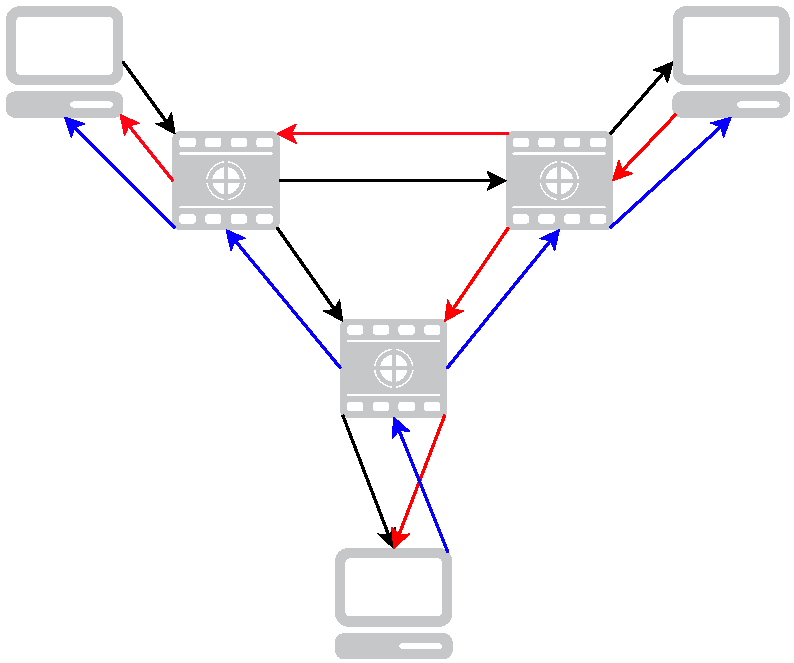
\includegraphics[width=0.7\textwidth]{./figures/mesh.pdf}
      \caption[Mesh topology for WebRTC]{Mesh topology for WebRTC.}
	\label{fig:meshTopology}
\end{figure}

Our topology, shown in Figure~\ref{fig:meshTopology}, consist in a mesh network of different virtual machines that connect by using our centralized {\it dialogue.io} application for signaling, media is sent over the peers directly, this will produce a big load in the performance for those clients as the amount of peer connections will be large, each of them obliged to encode and decode media, different from the previous example of parallel calls in this case all the peer connections will be running in the same process making the resource management a key point for the performance of WebRTC. We have increased the amount of CPUs to two in order to get proper results.

Three peers are used for the first test and it will increased by one peer every test, the output for the first test is shown in Table~\ref{fig:mesh_three_peers}. It is important to consider the amount of time required to set up the call, the worst result for the setup time in this scenario has been of 2206 ms to set up the three whole mesh. 

\begin{table}[h]
\begin{center}
    \begin{tabular}{c D{,}{\pm}{-1} D{,}{\pm}{-1} D{,}{\pm}{-1} }
   	 \toprule
	\textit{}
	& \multicolumn{1}{c}{\textit{Machine A}}
	& \multicolumn{1}{c}{\textit{Machine B}}
	& \multicolumn{1}{c}{\textit{Machine C}}\\
	\midrule
	\textbf{CPU (\%)} & 88.5 ,4.77 & 89.49 ,4.46 & 91.65 ,4.23\\
	\textbf{Memory (\%)} & 49.25 ,0.33 & 50.52 ,0.28 & 55.52 ,0.29\\
	\textbf{Bandwidth (Kbit/s)} & 333.38 ,115.13 & 344.48 ,95.43 & 410.77 ,115.97\\
	\bottomrule
    \end{tabular}
    \caption[CPU, memory and bandwidth results for three peer mesh scenario without relay]{CPU, memory and bandwidth results for three peer mesh scenario without relay.}
    \label{fig:mesh_three_peers}
\end{center}
\end{table}

CPU and memory usage is nearly double than in the previous scenario, considering we have doubled the CPU capacity, being this very consuming taking into consideration that is the only application running on the test machine.

Bandwidth will be an important constraint when having multiple peer connections, in a single P2P call we have two streams that are being sent/received, in mesh this amount is greater. Figure~\ref{fig:bwThreeMesh} represents the bandwidth mean and deviation for the three peer mesh call without relay, for every machine we will have two remote streams plotted with different bandwidth rates for them, is interesting to see how they are related in being one always greater than the other, this means that one stream will handle better quality than its other peer.

\begin{figure}[h]
  \centering
    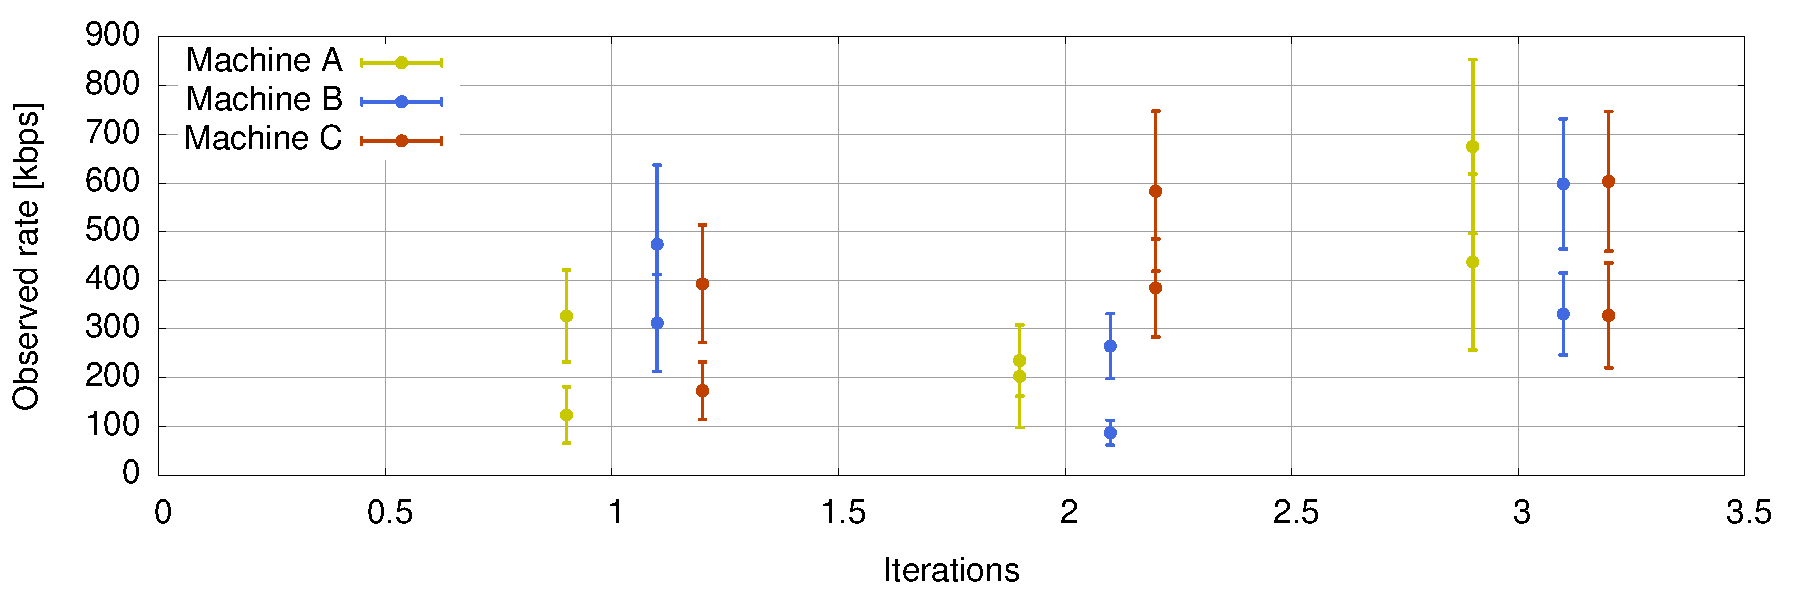
\includegraphics[width=1\textwidth]{./figures/mesh_mean_deviation_bw.pdf}
      \caption[Bandwidth average and deviation for three peers mesh call]{Bandwidth average and deviation for three peers mesh call.}
	\label{fig:bwThreeMesh}
\end{figure}

The total averaged bandwidth is approximately 362 Kbit/s, as it can be observed this value does not agree with the real plot for every peer (\ref{fig:bwThreeMesh}), this is due to the disturbances of the call and the continuous rate adaptation of the congestion mechanism. For better accuracy and understanding of what happened during the call we should look directly to the continuous rate of the incoming streams in Figure~\ref{fig:three_mesh}.

\begin{figure}[h]
        \centering
        \begin{subfigure}[b]{0.5\textwidth}
                \centering
                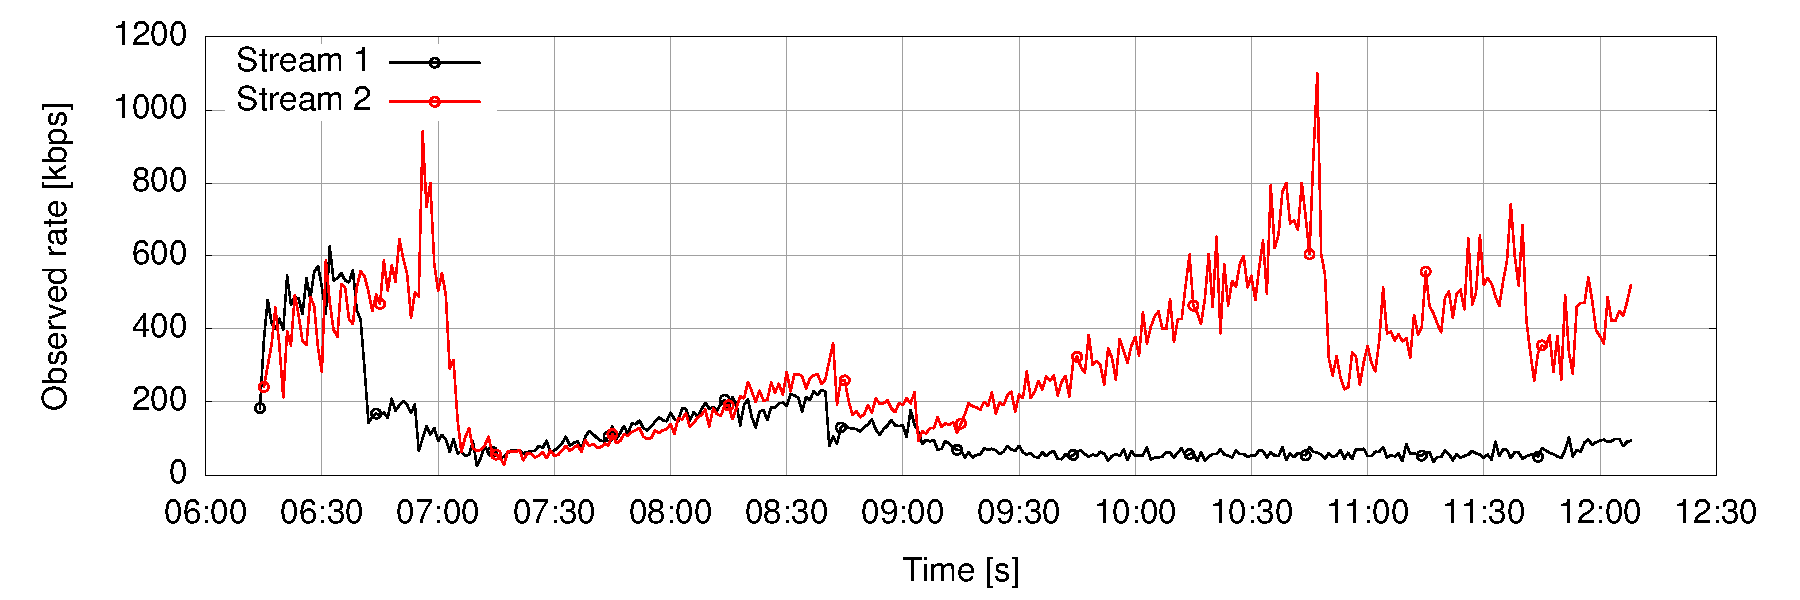
\includegraphics[width=\textwidth]{./figures/peer1_three_calls_bw.pdf}
                \caption{Remote streams for machine A}
                \label{fig:three_mesh_A}
        \end{subfigure}%
        ~ %add desired spacing between images, e. g. ~, \quad, \qquad etc.
          %(or a blank line to force the subfigure onto a new line)
        \begin{subfigure}[b]{0.5\textwidth}
                \centering
                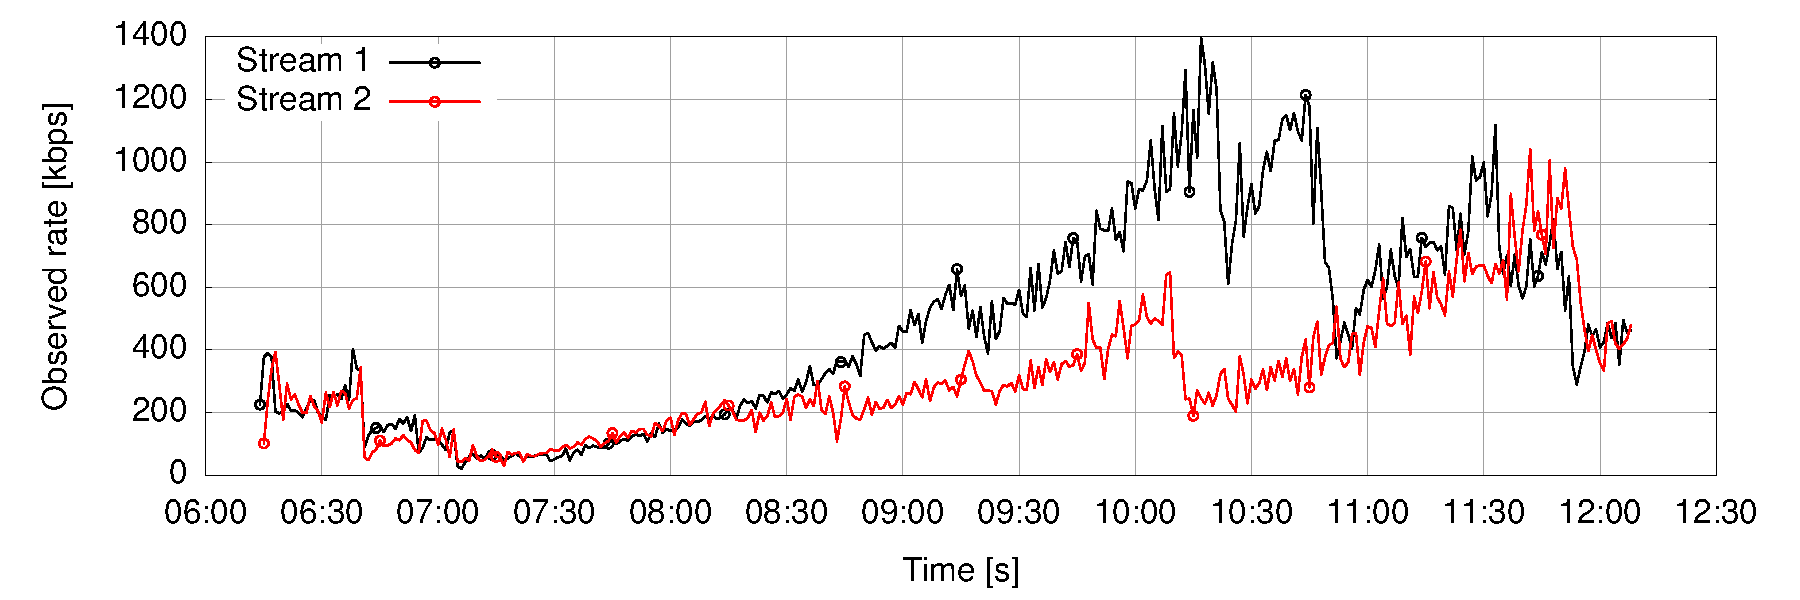
\includegraphics[width=\textwidth]{./figures/peer2_three_calls_bw.pdf}
                \caption{Remote streams for machine B}
                \label{fig:three_mesh_B}
        \end{subfigure}        
        ~ %add desired spacing between images, e. g. ~, \quad, \qquad etc.
          %(or a blank line to force the subfigure onto a new line)
        \begin{subfigure}[b]{0.5\textwidth}
                \centering
                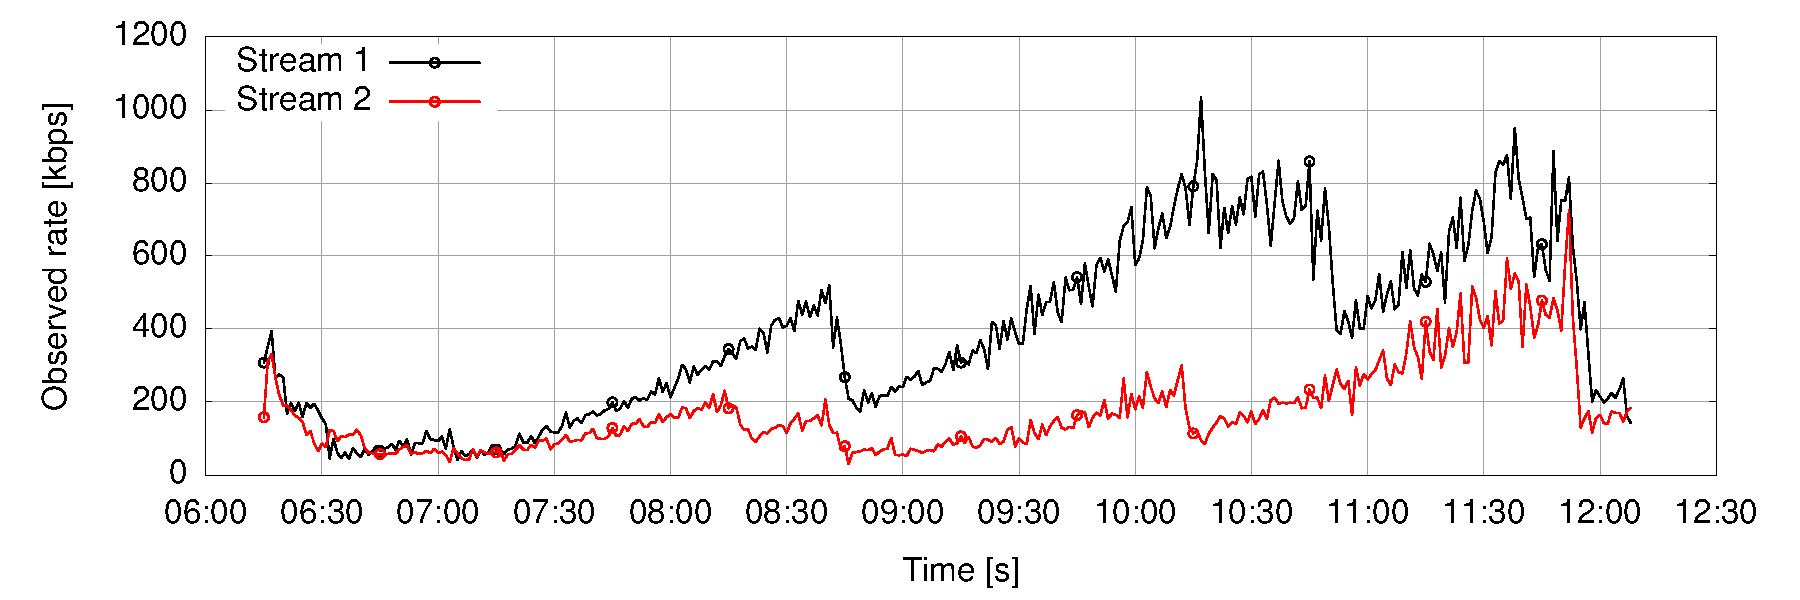
\includegraphics[width=\textwidth]{./figures/peer3_three_calls_bw.pdf}
                \caption{Remote streams for machine C}
                \label{fig:three_mesh_C}
        \end{subfigure}
        \caption[Bandwidth plot during all the call for the incoming streams of each peer for the first iteration]{Bandwidth plot during all the call for the incoming streams of each peer for the first iteration.}
        \label{fig:three_mesh}
\end{figure}

Each machine will have a pair of incoming streams, the rate calculated for the streams is based on the same mechanisms as the previous tests, this figure should look similar to Figure~\ref{fig:three_parallel} as they both are running multiple peer connections in the same test, we can see how the rate is being recalculated and how one of the streams is always being deprecated to a very low rate compared to the rest at a certain point when the other increase their throughput. This response of the rate adaptation will be negative to the call. 

Furthermore, a different behavior is observed in the delay of the call (Figure~\ref{fig:delay_mesh_peer1}), compared to the parallel calls (\ref{fig:three_parallel}) which had a very bad response to OWD in this specific case the output for the same four streams in delay is much better than the prior test.

\begin{figure}[h]
        \centering
        \begin{subfigure}[b]{0.5\textwidth}
                \centering
                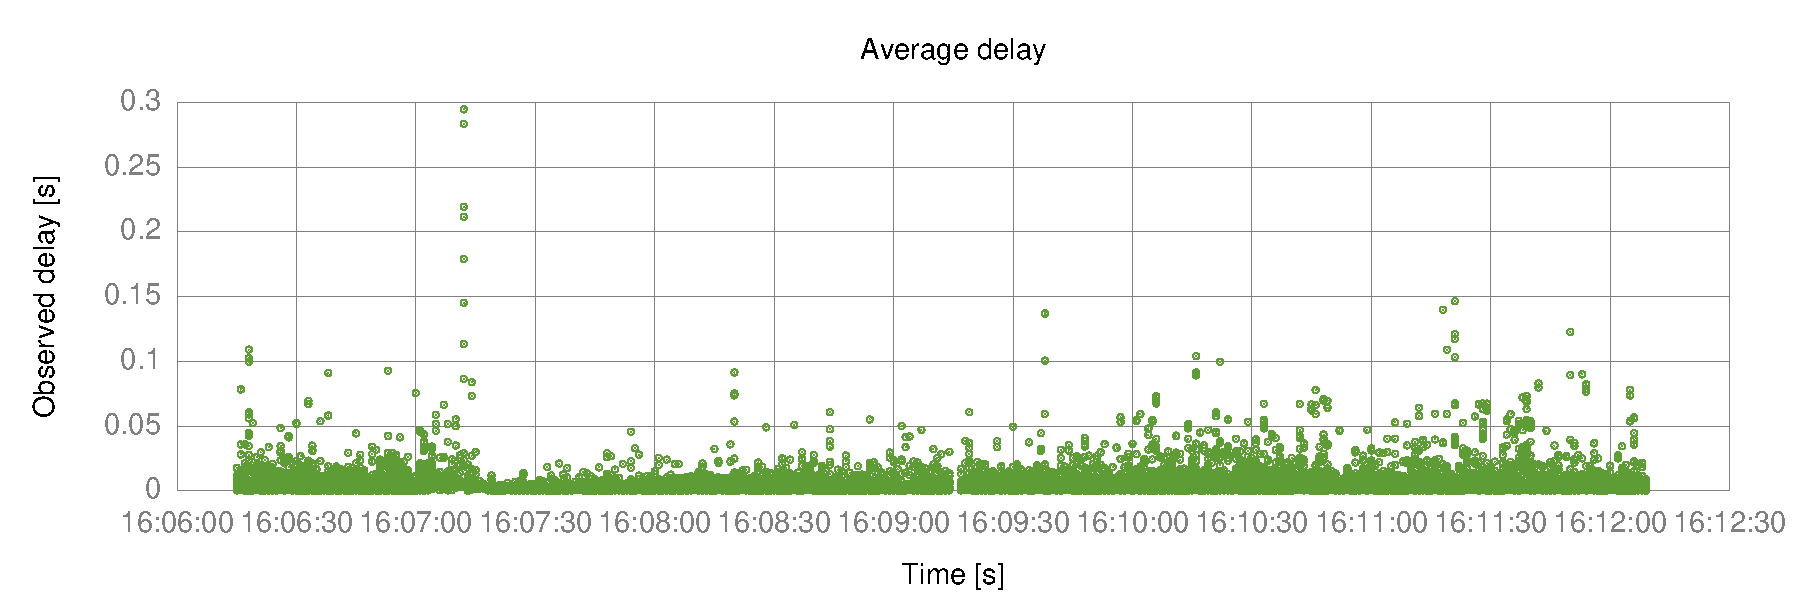
\includegraphics[width=\textwidth]{./figures/mesh_delay_1_116_6d141817.pdf}
                \caption{Delay for Figure~\ref{fig:three_mesh_A} stream 1}
                \label{fig:delay_mesh_peer1_1}
        \end{subfigure}%
        ~ %add desired spacing between images, e. g. ~, \quad, \qquad etc.
          %(or a blank line to force the subfigure onto a new line)
        \begin{subfigure}[b]{0.5\textwidth}
                \centering
                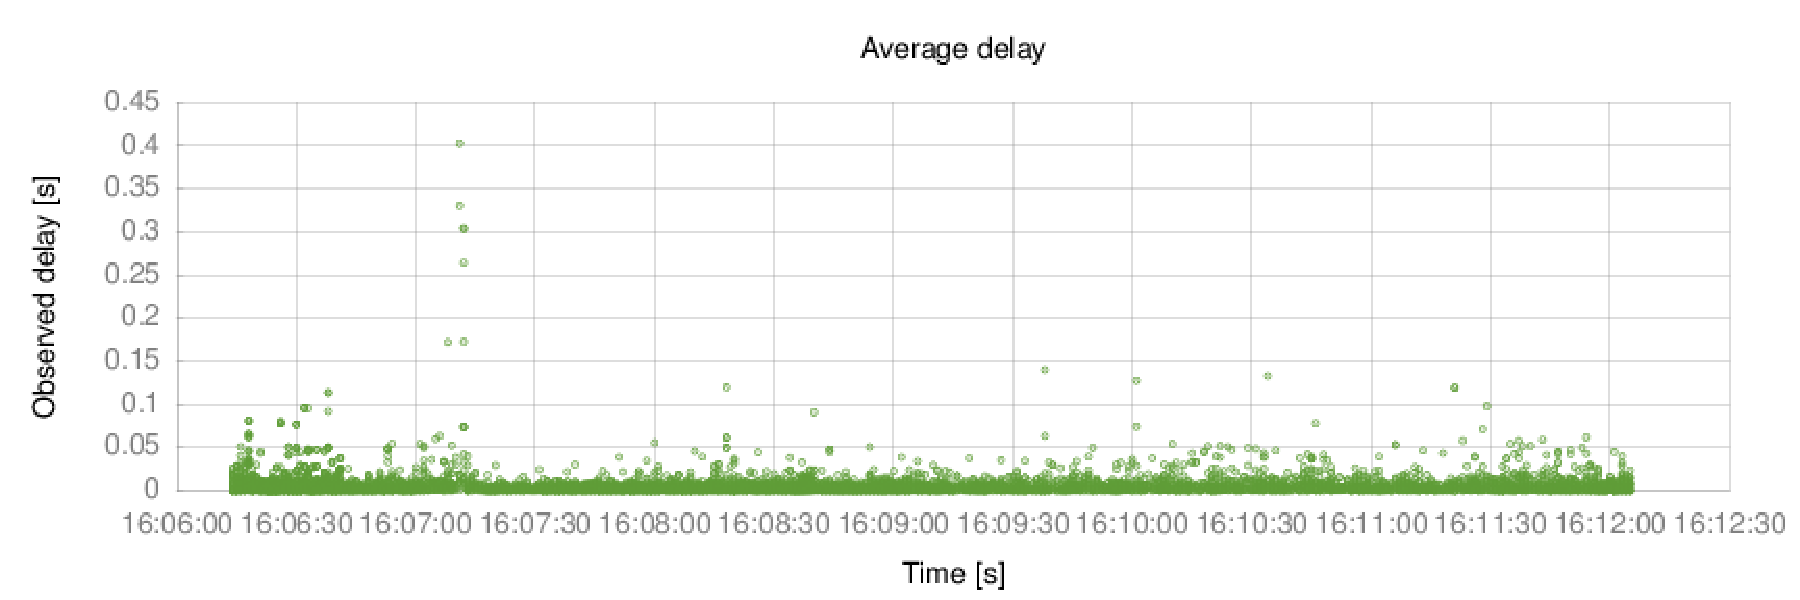
\includegraphics[width=\textwidth]{./figures/mesh_delay_1_116_c57d9b9b.pdf}
                \caption{Delay for Figure~\ref{fig:three_mesh_A} stream 2}
                \label{fig:delay_mesh_peer1_2}
        \end{subfigure}
        \caption[Delay output for Figure~\ref{fig:three_mesh_A} incoming streams]{Delay output for Figure~\ref{fig:three_mesh_A} incoming streams.}
        \label{fig:delay_mesh_peer1}
\end{figure}

The global delay distribution response is also good compared to previous tests, we can compare the obtained one in Figure~\ref{fig:delayThreeMesh} with the three parallel calls in Figure~\ref{fig:delayThreeCalls} and \ref{fig:delayThreeCallsAsync}. Considering the curve of the delay for the mesh networks we can say that the delay won't be affecting significantly the user experience during the call duration, we won't have good quality regarding the video and rate but there won't be any sudden delays expected in the communication. This means that from the perspective of a non relayed mesh call we can have three peers with relative acceptable bandwidth in most of the streams with an acceptable delay, the only drawback observed is the amount of used resources by the process, considering that the browser was the only application running on the test machine increasing the amount of processes will probably affect the behavior of the call.

\begin{figure}[h]
  \centering
    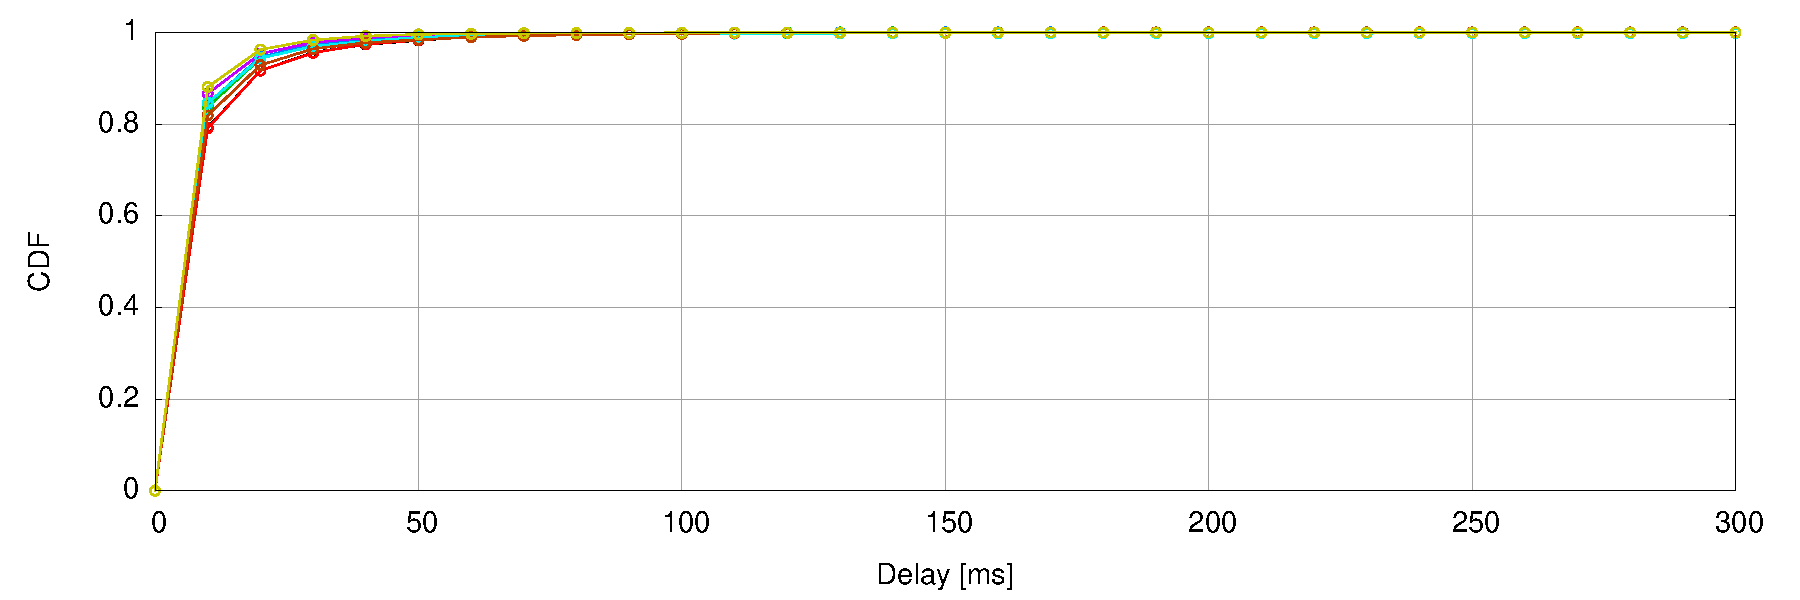
\includegraphics[width=1\textwidth]{./figures/mesh_total_delay_distribution.pdf}
      \caption[Total delay distribution for three peer mesh call without relay]{Total delay distribution for three peer mesh call without relay.}
	\label{fig:delayThreeMesh}
\end{figure}

Similar to the previous scenario we have run a test using the TURN as relay for the media to check the results, the bandwidth and CPU results are approximately the same, Figure~\ref{fig:delayThreeMeshNOTURN} represents the averaged delay result for the three iterations in both tests. Results are slightly better with the TURN, this might be due to the fixed path for routing the packets that produce smaller deviation, the averaged delay is similar in both cases.

\begin{figure}[h]
  \centering
    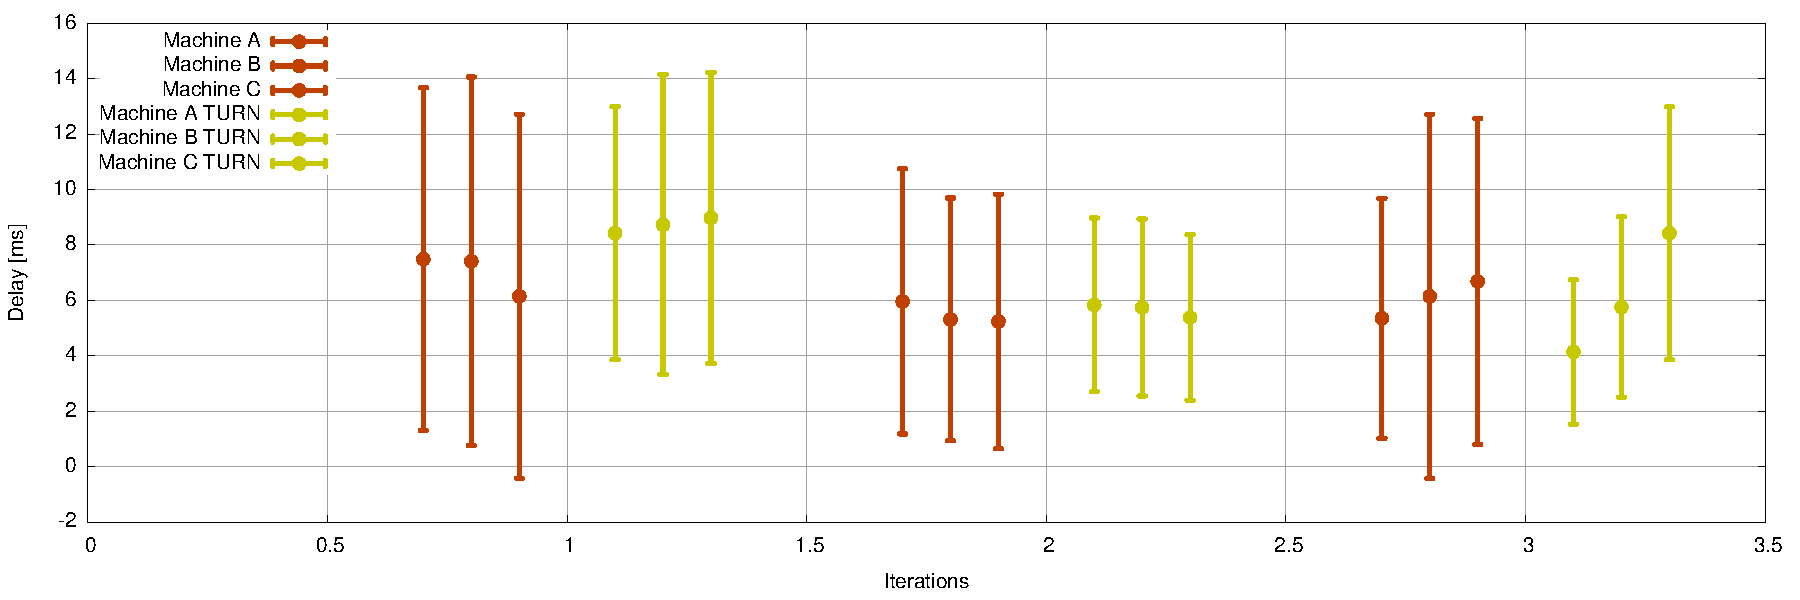
\includegraphics[width=1\textwidth]{./figures/mesh_turnno_mean_deviation_delay.pdf}
      \caption[Averaged delay and deviation for TURN and non relayed mesh call for all iterations]{Averaged delay and deviation for TURN and non relayed mesh call for all iterations.}
	\label{fig:delayThreeMeshNOTURN}
\end{figure}

For environments such as mesh, the usage of MCU should be considered as a good alternative to the pure P2P option, this could drastically reduce the resource consumption and bandwidth distribution on the different peer connections when using multiple peer topologies.

%\subsection{CPU performance}
%
%After running all the tests we can see that WebRTC is facing a big problem when it comes to CPU and memory consumption. Averaged computers could have problems when handling multiple peer connections in WebRTC, we have also tested the CPU usage in all those different scenarios. 

\subsection{Summary of results}

After all the performed tests we can conclude that WebRTC is a young protocol for real time communication that still has long way to go in terms of congestion control to adapt to all topologies, still is a reliable and interesting method that uses all existing technologies previously developed for other projects there is a lot of work to do in terms of scalability and environment adaption. 

Considering the existing WebRTC congestion mechanisms we can conclude that is still not ready for low tolerance networks or to be used simultaneously in different calls, the resource consumption of the existing WebRTC API is still something to care if we want to integrate WebRTC in mobile devices.

In multiple peer connections environments the usage of an MCU is something that should be considered in order to reduce load and increase performance, the actual WebRTC API does not allow to natively use multiplexing of streams over the same peer connection but the roadmap of the standardization protocol includes this feature for future versions of WebRTC.

Delay response for some low latency environments is not suitable for production applications and scenarios should be considered  by developers prior deciding to use WebRTC instead of other competitors.